
\chapter{Theory}
\label{ch:Theory}

In this chapter a theoretical background will be presented on the Standard Model of particle physics with special attention paid to the top quark's properties and decays.  This will include discussion of all of the fundamental particles and their interactions through the fundamental forces of nature: electromagnetism and the strong and weak nuclear forces.

%%%%%%%%%%%%%%%%%%%%%%%%%%%%%%%%%%%%%%%%%%%%%%%
%%%%%%%%%%%%%%%%%%%%%%%%%%%%%%%%%%%%%%%%%%%%%%%
\section{The Standard Model Particles}
\label{SMParticles}
The Standard Model of particle physics is the cornerstone of our understanding of the basic building blocks of nature and their interactions.  Typical matter is made up of atoms consisting of electrons around an inner nucleus of protons and neutrons.  These protons and neutrons are made up of a collection of up and down type quarks along with sea quarks and gluons.  Protons consist of two up type quarks and a down type quark, while neutrons contain two down type quarks and a single up type quark.  

Within the Standard Model all matter (quarks and leptons) is made up of fermions (spin-$\frac{1}{2}$ particles).  In addition to the up and down type quarks and the electron the remaining fermions can be decribed as additional `generations' that are similar, each consisting of two quarks and a lepton.  Every generation consists of quarks with electric charge $+\frac{2}{3}$ and $-\frac{1}{3}$ and a lepton with charge $-1$ along with an electrically neutral lepton called a neutrino.  All of these fermions are listed in Table \ref{tab:SM}.  

While we can observe the leptons in nature, free quarks do not exist.  We can observe quarks only as part of a bound state called a hadron.  If a hadron consists of a quark-antiquark pair ($q\bar{q}$) it is called a meson.  Sets of three quarks or three antiquarks ($qqq$ or $\bar{q}\bar{q}\bar{q}$) are called baryons.  Protons and neutrons are baryonic matter.

In addition to the fermions the Standard Model contains gauge, or vector, bosons which are spin-1 particles that carry the fundamental forces of nature.  The electromagnetic force is mediated by the massless, charge neutral photon ($\gamma$). The nuclear weak force is carried by two massive bosons: the electrically neutral Z boson and the charged ($\pm 1$) W boson.  These bosons together dictate electroweak interactions within the Standard Model.  The remaining force, the nuclear strong force, is carried through the gluon ($g$).  Gluons are massless and chargeless but carry color, an analog of electric charge in the electroweak interaction.  The last remaining piece of the Standard Model is the scalar (spin-0) Higgs boson.  This Higgs boson is a massive electrically neutral boson that is responsible for giving mass to the massive fundamental particles.  All of these bosons are also shown in Table \ref{tab:SM}.  

\begin{table}[h]
\begin{center}
\footnotesize
\begin{tabular}[h]{|c||c|c|c|c|}
\hline
 & Particle & Spin & Charge & Mass \\
\hline\hline
Quarks &&&&\\
\hline
u type &u& & &${2.4^{+0.6}_{-0.4} \text{ MeV}}$\\
 &c&${\frac{1}{2}}$&${\frac{2}{3}}$&${1.28\pm{0.03} \text{ GeV}}$\\
 &t& & &${173.1\pm{0.6} \text{ GeV}}$\\
\hline
d type & d& & & ${4.7^{+0.5}_{-0.4} \text{ MeV}}$\\
 & s & ${\frac{1}{2}}$ & ${-\frac{1}{3}}$ & ${96^{+8}_{-4} \text{ MeV}}$\\
 & b & & & ${4.18^{+0.04}_{-0.03} \text{ GeV}}$\\
\hline\hline
Leptons &&&&\\
\hline
e doublet & e & ${\frac{1}{2}}$ & -1 &${0.5109989461\pm{}0.000000003 \text{ MeV}}$\\
 & ${\nu_{e}}$ & & 0 & ${< 2 \text{ eV}}$\\
 \hline
${\mu}$ doublet & ${\mu}$ & ${\frac{1}{2}}$ & -1 &${105.6583745\pm{}0.0000024 \text{ MeV}}$\\
 & ${\nu_{\mu}}$ & & 0 & ${< 2 \text{ eV}}$\\
 \hline
${\tau}$ doublet & ${\tau}$ & ${\frac{1}{2}}$ & -1 &${1776.86\pm{}0.12 \text{ GeV}}$\\
 & ${\nu_{\tau}}$ & & 0 & ${< 2 \text{eV}}$\\
 \hline\hline
 Bosons &&&&\\
 \hline
 Vector & ${\gamma}$ & 1 & 0 & ${< 10^{-18} \text{ eV}}$\\
 & ${g}$ & 1 & 0 & ${0}$\\
 & ${W}$ & 1 & ${\pm}$ & ${80.385\pm{}0.0015 \text{ GeV}}$\\
 & ${Z}$ & 1 & 0 & ${91.1876\pm{}0.0021 \text{ GeV}}$\\
 \hline
 Scalar & H & 0& 0 & ${125.09\pm{}0.21\pm{}0.11 \text{ GeV}}$\\
 \hline
\end{tabular}
\caption[Particles of the Standard Model.]{Particles of the Standard Model\cite{PDG2018}. It should be noted that the quark masses should not be considered too precise as they are hard to define due to quark confinement\cite{QuarkConfinement} the u, c, d, s, and b cannot be isolated independently and are implied indirectly through scattering experiments and are heavily model dependent.}
\label{tab:SM}
\end{center}
\end{table}


%%%%%%%%%%%%%%%%%%%%%%%%%%%%%%%%%%%%%%%%%%%%%%%
%%%%%%%%%%%%%%%%%%%%%%%%%%%%%%%%%%%%%%%%%%%%%%%
\section{The Standard Model Interactions}
In addition to describing these particles the Standard Model also describes the ways in which these particles are capable of interacting.  All of the particles decribed in the previous section are included in the following theory.  The Standard Model Lagrangian is simply a function of fields and their derivatives taken at one point in spacetime, $x^{\mu}$.  
 \[ \mathcal{L} \lbrack \phi_{i}(x),\partial_{\mu}\phi_{i}(x) \rbrack \] 
The Standard Model is defined having a gauge symmetry
\[ G_{SM} =SU(3)_C \times SU(2)_L \times U(1)_Y \]
where all of the particle content descibed in Section \ref{SMParticles} is described under this symmetry in Table \ref{tab:SMGaugePart}\cite{GrossmanLecture}.  The eight color-anticolor combinations of spin-1 gluons are associated with $SU(3)_C$ where the C denotes `color' quantum numbers of the gauge group.  Any particle that carries color will interact with gluons via the strong nuclear interaction.  The three spin-1 gauge bosons $W_a$, $a=1,2,3$ conduct the weak isospin $SU(2)_L$ symmetry where the L denotes that only left-handed chiral fermions transform with respect to this symmetry.  The left-handed fermions are $SU(2)$ doublets while the right-handed components are singlets.  The remaining spin-1 gauge boson, B, is associated with $U(1)^Y$ weak hypercharge.  
\begin{table}[]
\begin{center}
\begin{tabular}{|c|c|c|c|}
 \hline
Name             & Field Components    & $(SU(3)_C, SU(2)_L, U(1)_Y)  $  &   Comments                            \\   \hhline{====}
\multicolumn{4}{|c|}{Spin-1/2 Quarks} \\ \hline
Q 		&($u_L$  $d_L$)          &   (3,2,$\frac{1}{6}$)		&			\\
	           &$u_R$          	    &	(3,1,$\frac{2}{3}$)		&   x3 generations \\
           	&$d_R$		    &    (3,1, $-\frac{1}{3}$)           &           		\\
\hhline{====}
\multicolumn{4}{|c|}{Spin-1/2 Leptons}\\ \hline
L 		&($\nu_L$  $e_L$)          &   (1,2,$-\frac{1}{2}$)		&			\\
	           &$e_R$          	    &	(1,1,$-1$)		&   x3 generations \\
\hhline{====}
\multicolumn{4}{|c|}{Spin-0 Higgs}\\ \hline
$\phi$ 		&($\phi^{+}$  $\phi^0$)          &   (1,2,$\frac{1}{2}$)		&			\\
\hhline{====}
\multicolumn{4}{|c|}{Spin-1 Gauge Bosons} \\ \hline
Gluons 	& $G^{1,...,8}$          	      &   (8,1,0)		&			\\
W       		&($W^1$ $W^2$  $W^3$)     &	(1,3,0)		&   			 \\
B          	&$B^0$		    &    (1,1,0)           &           				\\
\hhline{====}
\end{tabular}
	\caption{Summary of the Standard Model field contents and their representations in the gauge group, labeled by their dimension ($SU(3)_C$ and $SU(2)_L$) and weak hypercharge ($U(1)_Y$).}
	\label{tab:SMGaugePart}
\end{center}
\end{table}


The $W^\pm$, $Z$, and photon ($\gamma$) are produced by spontaneous symmetry breaking $SU(2)_L \times U(1)_Y$ implied by the Higgs potential discussed Section \ref{sec:EWSB}.

 One general way of expressing the Standard Model Lagrangian is 
\[
\mathcal{L}_{SM} = \mathcal{L}_{kinetic}+\mathcal{L}_{Higgs}+\mathcal{L}_{Yukawa}
\]
where we have a kinetic term for the bosons and fermions, a Higgs term which includes the Higgs kinetic term and potential, and a term that dictates the Yukawa interactions.  This can be expanded out
\[ \mathcal{L} = (-\frac{1}{4} F_{\mu\nu}F^{\mu\nu} + i \bar{\psi}\slashed{D}\psi +\text{h.c.} ) + (|D_{\mu}\phi|^2+V(\phi)) + (\psi_i Y_{ij}\psi_j \phi +\text{h.c.})
\]
All of the gauge field strengths are included within $F_{\mu\nu}$.  To maintain gauge invariance for the kinetic terms the derivative must be replaced by the covariant derivative 
\[ \partial^\mu \rightarrow D^\mu = \partial^\mu +ig_s G^{\mu}_a L_a + i g W^{\mu}_a T_a +i g' B^\mu Y
\]

The eight gluon fields are described by $G^{\mu}_a$, the three weak interaction boson fields are decribed by $W^{\mu}_a$, and the hypercharge boson field is $B^{\mu}$.  Here $g_s$, $g$, and $g'$ are the gauge coupling constants, and $L_a$, $T_a$, and $Y$ are the generators for $SU(3)_C$, $SU(2)_L$, and $U(1)_Y$ respectively.   The generators are described by the Gell-Man matricies for $L_a$ ($\frac{1}{2}\lambda_a$ for triplets, 0 for singlets), the Pauli matricies for $T_a$($\frac{1}{2}\sigma_a$ for doublets, 0 for singlets), and the $U(1)_Y$ charges for $Y$.


%%%%%%%%%%%%%%%%%%%%%%%%%%%%%%%%%%%%%%%%%%%%%%%
%%%%%%%%%%%%%%%%%%%%%%%%%%%%%%%%%%%%%%%%%%%%%%%

\section{Electroweak Symmetry Breaking}
\label{sec:EWSB}
  The spin-1 particles within the Standard Model are massless; however we know that the real bosons made up of these states are massive (i.e. the $W^\pm$ and $Z$).  This comes about from a spontaneous symmetry breaking of $SU(2)_L \times U(1)_Y$ by a particle whose ground state is not invariant under the symmetry.  The scalar Higgs field is capable of doing this while at the same time not breaking the $SU(3)_C$ symmetry leaving the gluons massless because $\phi$ is an $SU(3)_C$ singlet.

Expanding the Yukawa term of the Lagrangian we see that the covariant derivative of the scalar field becomes
\[ D_{\mu} \phi = \partial_\mu \phi - \frac{i}{2}(gW_{\mu}^{a} \frac{\sigma^a}{2}+g' B_\mu)\phi
\]
and the potential
\[ V(\phi) = \lambda (\phi^{\dagger} \phi - \frac{\mu^2}{2 \lambda})^2 = \lambda(\phi^\dagger \phi)^2 -\mu^2 \phi^\dagger \phi + \frac{\mu^4}{4\lambda}
\]

It follows that if $\frac{\mu^2}{\lambda}>0$ then this potential has a non-zero vacuum expectation value $v^2 \equiv \frac{\mu^2}{\lambda}$.  The condition $\lambda>0$ is a requirement on the vacuum stability of the model such that $\mu^2 <0$ is the requirement for spontaneous symmetry breaking.  Therefore we can make a gauge transformation such that 
\[ \left<{\phi}\right>=\frac{1}{\sqrt{2}}\begin{pmatrix} 0\\v\end{pmatrix}
\]

\subsection{Gauge Boson Masses}
The mass eigenstates of the spin-1 bosons can be recovered from this by writing out the mass part of the gauge boson kinetic term $|D^\mu \phi|^2$
\[ \mathcal{L}_{mass} = -\frac{1}{8}\begin{pmatrix} 0 & v\end{pmatrix}\begin{pmatrix}gW_3+g' B & g(W_1 -iW_2)\\g(W_1+iW_2) & -gW_3+g'B\end{pmatrix}^2\begin{pmatrix}0\\v\end{pmatrix}
\]
and if we define the weak mixing angle as $\text{tan}\theta_W \equiv \frac{g'}{g}$ and the mass eigenstates of the bosons
\[W^\pm\equiv\frac{1}{\sqrt{2}}(W_1\mp iW_2)\]
\[Z \equiv \text{cos}\theta_W W_3 -\text{sin}\theta_W B\]
\[A \equiv \text{sin}\theta_W W_3 +\text{cos}\theta_W B\]

then the mass matrix can be diagonalized to give 
\[ \mathcal{L}_{mass} = -\frac{1}{4} g^2 v^2 W^+ W^- -\frac{1}{8}(g^2 + g'^2)v^2 Z^2 \]
which gives us the masses of our bosons: $M_W^2 = \frac{1}{4}g^2 v^2$, $M_Z^2=\frac{1}{4}(g^2 +g'^2)v^2$, and $M_A^2=0$.  Since the field A is massless there is an unbroken $U(1)$ that is identified as the photon and $U(1)_{EM}$.

%%%%%%%%%%%%%%%%%%%%%%%%%%%%%%%%%%%%%%%%%%%%%%%
\subsection{Fermion Masses}
Fermions acquire their masses from the Yukawa term in the Lagrangian.  If we transform into the mass basis, also using the replacement of the scalar field corresponding to a physical Higgs boson
\[ \phi=\frac{1}{\sqrt{2}}\begin{pmatrix}0\\v+H(x)\end{pmatrix} \]
then we can write the $SU(2)_L$ quark doublets into their components \[Q_{Li}=\begin{pmatrix}U_{Li}\\D_{Li}\end{pmatrix}\]
The Yukawa term can be broken down into a baryonic and leptonic portion.  The lepton portion leads to charged lepton masses after the Higgs acquires a vacuum expectation value after electroweak symmetry breaking.
\[ -\mathcal{L}^\text{leptons}_\text{Yukawa} = Y_{ij}^e \overline{L_{Li}}\phi E_{Rj} \]
This leads to three physical parameters, which are generally chosen to be the three charged lepton masses (electron, muon, tau).  The baryonic term leads to quark masses and flavors. Ten physical parameters arise from the baryonic Yukawa interactions  
\[ -\mathcal{L}^{\text{quarks}}_\text{Yukawa} = Y_{ij}^d \overline{Q_{Li}} \phi D_{Rj} + Y_{ij}^u \overline{Q_{Li}} \tilde{\phi}U_{Rj} + \text{h.c.}\]
Expanding this in terms of the above $SU(2)_L$ components
\[-\mathcal{L}=(M_d)_{ij}\overline{D_{Li}} D_{Rj} +(M_u)_{ij}\overline{U_{Li}}U_{Rj} +\text{h.c.} \]
such that $M_q = \frac{v}{\sqrt{2}}Y^q$.  Unitary matricies ($V_{qL}$ and $V_{qR}$) that take us to the mass basis can always be found. 
\[V_{qL} M_q V_{qR}^{\dagger} =M_q^\text{diag}, \text{  for q=u,d} \]
The quark mass eigenstates that follow from this are: \[q_{Li}=(V_{qL})_{ij}q_{Lj}^I \text{  and  } q_{Ri} = (V_{qR})_{ij}q_{Rj}^I \] being transformed from the interaction basis $I$.

%%%%%%%%%%%%%%%%%%%%%%%%%%%%%%%%%%%%%%%%%%%%%%%
\subsection{The CKM Matrix}
\label{sec:CKM}
In the interaction basis interactions between quarks and $W^\pm$ come from the $\bar{\psi}\slashed{D}\psi$ kinetic term in the Lagrangian.  We can explicitly write this out in both the interaction and mass basis such that:
\[\text{Interaction Basis: } -\mathcal{L}^q_{W^\pm} =\frac{g}{2}\overline{Q_{Li}}\gamma^{\mu}W_{\mu}^a\tau^a Q_{Li} +\text{h.c.}\]
\[\text{Mass Basis: } -\mathcal{L}^q_{W^\pm} =\frac{g}{\sqrt{2}}\begin{pmatrix}\bar{u}_L &\bar{c}_L &\bar{t}_L\end{pmatrix}\gamma^\mu (V_{uL}V_{dL}^{\dagger})_{ij}W_{\mu}^+ \begin{pmatrix} d_L \\s_L \\b_L\end{pmatrix}+\text{h.c.} \]
The term $V=V_{uL}V_{dL}^{\dagger}$ in the previous equation is a unitary $3\times3$ matrix known as the Cabibbo-Kobayashi-Maskawa (CKM) matrix \cite{CKM1,CKM2} that describes quark mixing.  The CKM matrix can be expressed simply:
\[
V_{CKM} = 
\begin{bmatrix}
V_{ud} & V_{us} & V_{ub} \\
V_{cd} & V_{cs} & V_{cb} \\
V_{td} & V_{ts} & V_{tb}
\end{bmatrix}
\]
The components of the CKM matrix are not all arbitrary.  This can be expressed in the Wolfenstein parametrization\cite{Wolfenstein} to show that there are only four parameters, three real and one complex.  The Wolfenstein parameterization is an expansion in $V_{us}=\lambda= 0.2257^{+0.009}_{-0.0010}$. Where $A=0.814^{+0.021}_{-0.022}$, $\rho=0.135^{+0.031}_{-0.016}$, and $\eta = 0.349^{+0.015}_{-0.017}$ \cite{PDG2018}.
\[
V_{CKM}^\text{Wolfenstein} = 
\begin{bmatrix}
1-\frac{1}{2}\lambda^2 	& \lambda			  & A \lambda^3(\rho - i \eta) \\
-\lambda 			& 1-\frac{1}{2}\lambda^2	  & A\lambda^2 \\
A\lambda^3(1-\rho -i\eta) & -A \lambda^2		 & 1
\end{bmatrix}
\]

This formulation demonstrates quite clearly that the CKM matrix is almost diagonal but has small off-diagonal terms.  This means that interactions between quarks is strongest within a generation i.e., up and down quarks, charm and strange quarks, and top and bottom quarks experience the largest degree of mixing between each other.  A top quark directly decays to a bottom quark and W boson almost all of the time ($\approx 99.83\%$ of the time).  While the mixing does not prohibit decaying to a strange or down quark instead of a bottom, it is a significantly rarer event ($\approx 0.16\%$ and $\approx 0.01\%$, respectively).  The values for all of these parameters have been measured experimentally and are collected by the Particle Data Group\cite{PDG2018}: 

\[ V_{CKM} =
\begin{bmatrix}
0.97420 \pm 0.00021 & 0.2243 \pm 0.0005 & 0.00394 \pm 0.00036 \\ 
0.218 \pm 0.004 & 0.997 \pm 0.017 & 0.0422 \pm 0.0008 \\
0.0081 \pm 0.0005 & 0.0394 \pm 0.0023 & 1.019 \pm 0.025 
\end{bmatrix}
\]


%%%%%%%%%%%%%%%%%%%%%%%%%%%%%%%%%%%%%%%%%%%%%%%
%%%%%%%%%%%%%%%%%%%%%%%%%%%%%%%%%%%%%%%%%%%%%%%
\section{The Top Quark}

This dissertation will pay particular interest to the top quark, the heaviest of all of the fundamental particles, over 40 times heavier than its generational partner the bottom quark and $40\%$ larger than the Higgs boson, the next heaviest particle.  One of its most interesting properties, due to its large mass, is that it has an extremely small lifetime ($\approx 5 \times 10^{-25} s$).  This lifetime is orders of magnitude shorter than the characteristic time over which the strong nuclear interaction takes place ($\approx 10^{-23}s$), meaning that it decays before it can hadronize by combining with another quark to form a mesonic or baryonic system.  This allows us to observe the decays of the top quark directly as opposed to the decay products of a top quark system.
The top quark was first proposed as an explanation of CP violation in kaon decays by Kobayashi and Maskawa in 1973\cite{CKM2} which predicted a third generation of quarks.  At the time there was little evidence for this.  The later discovery of the charm quark, which was predicted to exist due to a suppresion caused by the GIM mechanism\cite{GIM} and formed the foundation of Kobayashi and Maskawa's work, provided further evidence.  The discovery of the charm filled out a complete 2 generation Standard Model (up, down, strange, and charm quarks and the electron and muon).  However the further observation of the tau lepton meant that the symmetry between lepton and quark generations would be broken without the existence of a third generation of quarks, the top and bottom, providing soft evidence of a third generation of quarks.  Within just a few years, in 1977, the bottom was also discovered\cite{BDiscovery} and the theoretical predictions of the Standard Model at the time heavily favored the existence of a 6th quark, the 3rd and heaviest up-type quark.  

%%%%%%%%%%%%%%%%%%%%%%%%%%%%%%%%%%%%%%%%%%%%%%%
\subsection{Discovering The Top Quark}

Almost 20 years went by after the discovery of the bottom quark and many experiments came up empty handed even while discovering the W and Z bosons (the Super Proton Synchrotron at CERN) before direct evidence for the top quark was observed at Fermilab's Tevatron in both the CDF and D0 experiments in 1995\cite{TopObs,TopObsD0}.  While the Tevatron only operated at a maximum energy of 1.96 TeV during its lifetime, further properties of the top quark could not be probed in detail due to a lack of statistics.  Not until the LHC began operation at a center of mass energy of 7 TeV in 2010 were enough top quarks produced to study the details of its interactions. 
\begin{figure}[h!]
	\centering
	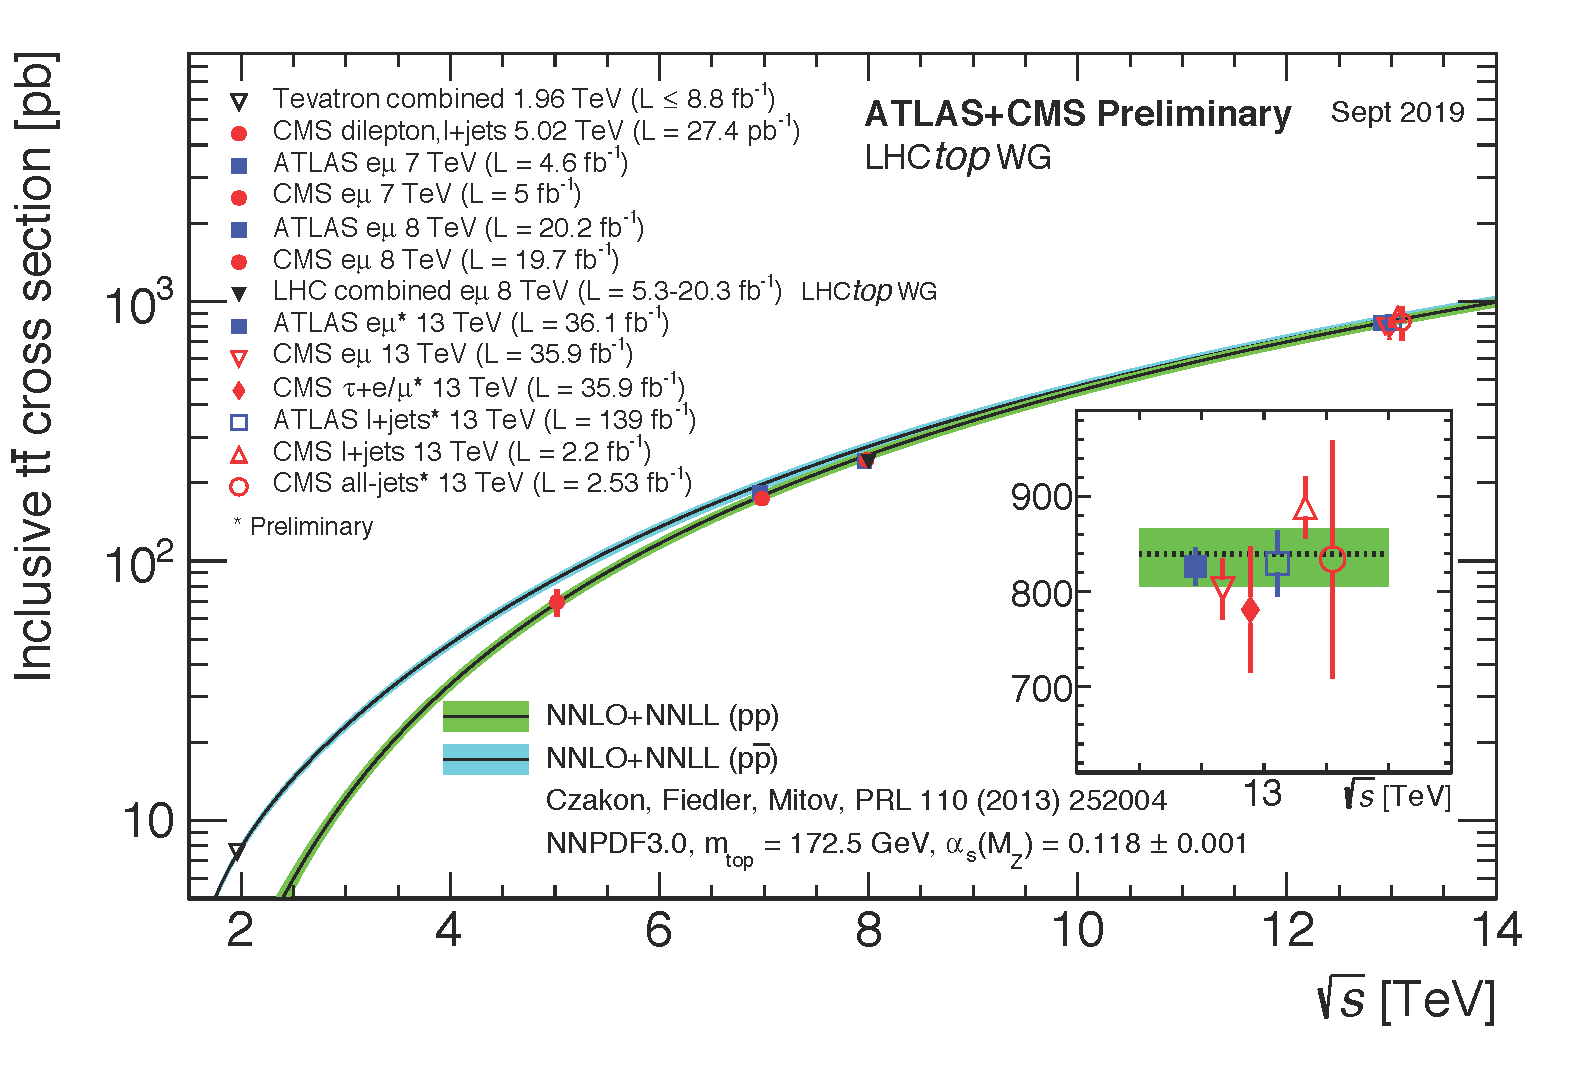
\includegraphics[width=\columnwidth]{../ThesisImages/Theory/ttprodxsec.png}
	\caption[Summary of $t\bar{t}$ production cross sections as a function of center of mass energy at Fermilab's Tevatron and CERN's LHC.]{Summary of $t\bar{t}$ production cross sections as a function of center of mass energy at Fermilab's Tevatron and CERN's LHC.  For a top mass of 172.5 GeV and center of mass energy of 13 TeV the central value cross section is calculated to be 831 pb\cite{TopWG}. }
	\label{fig:ttbarXSec}
\end{figure}

\begin{figure}[h!]
	\centering
	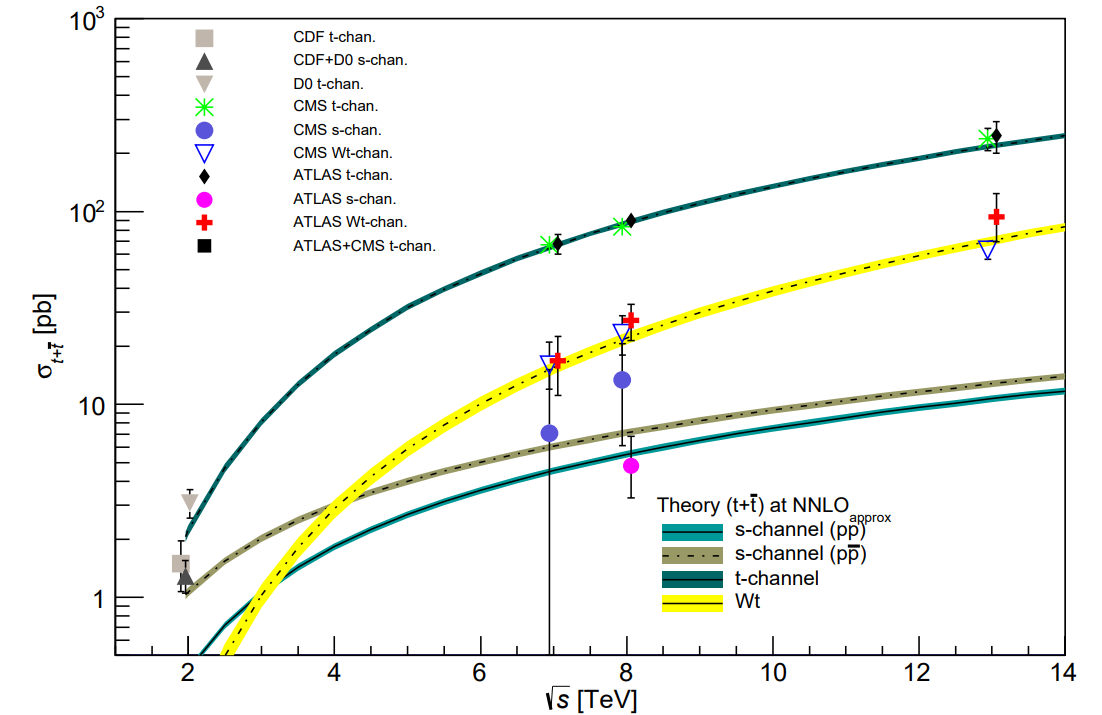
\includegraphics[width=\columnwidth]{../ThesisImages/Theory/singtprodxsec.png}
	\caption[Summary of single-top production cross sections as a function of center of mass energy at Fermilab's Tevatron and CERN's LHC.]{Summary of single-top production cross sections as a function of center of mass energy at Fermilab's Tevatron and CERN's LHC\cite{TopWG}.}
	\label{fig:singtXSec}
\end{figure}

 The amount of top quarks produced scale up by the energy as seen in Figure \ref{fig:ttbarXSec} as well as the integrated luminosity, or number of events produced, of the accelerator and detector setup.  The LHC has significantly more of both than the Tevatron did.  Throughout the entirety of Run-2 at the LHC there are expected to be more than 115,000 top pair events produced within the ATLAS detector, allowing physicists to probe the details of the top quark better than ever before.  


\subsection{Production and Decay At Hadron Colliders}

There are multiple ways to produce top quarks at the LHC.  The most prevelant production mechanism of top quarks is through producing top/anti-top quark pairs.  This can be done, to leading order, either by quark-antiquark annihilation (Figure \ref{fig:LOprod}a) or gluon gluon fusion (Figure \ref{fig:LOprod}b-d).  At the Tevatron, a proton anti-proton collider, the leading diagram was quark-antiquark annihilation because of the significantly larger amount of antiquarks in the collisions.  At the LHC the major production mechanism is gluon-gluon fusion, $\approx 90\%$, while quark-antiquark annihilation accounts for only $\approx 10\%$  of top quark pair production.  This is a strong interaction process and is therefore quite common.  The cross sections are shown in Figure \ref{fig:ttbarXSec}.

\begin{figure}[h!]
	\centering
	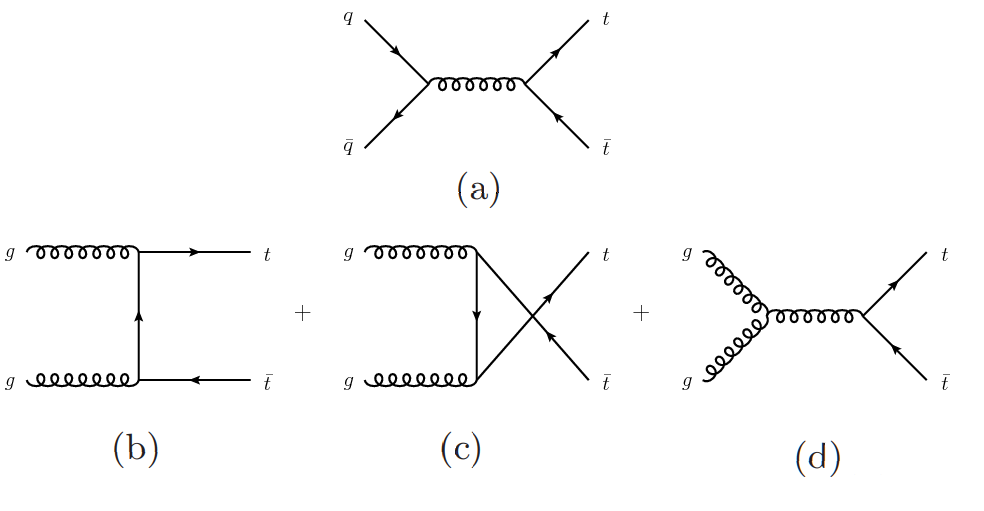
\includegraphics[width=\columnwidth]{../ThesisImages/Theory/LOPairProdDiags.png}
	\caption[Leading order diagrams for $t\bar{t}$ production at hadron colliders.]{Leading order diagrams for the production of top/anti-top quark pairs at hadron colliders.  Quark-antiquark annihilation diagram is shown in (a) while (b)-(d) show various gluon-gluon fusion diagrams.}
	\label{fig:LOprod}
\end{figure}

Single top quarks can also be produced through weak interactions, which is less common, and the leading diagrams are shown in Figure \ref{fig:LOprodSing} and their cross sections as measured at the LHC and Tevatron are shown in Figure \ref{fig:singtXSec}.  Comparing the leading production mechanisms at 13 TeV, it can be seen that $t\bar{t}$ production is about a factor of 4 larger than single top production.  This means there are about 8x as many top quarks looking at pair produced events, as two are produced per event while giving an additional experimental handle in looking for an invariant mass of final state products around the top quark mass.

\begin{figure}[h!]
	\centering
	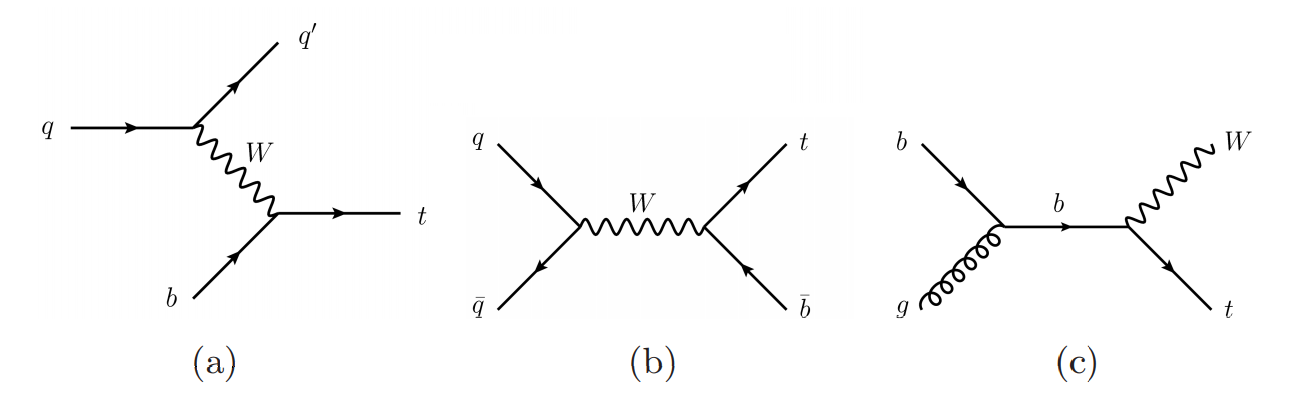
\includegraphics[width=\columnwidth]{../ThesisImages/Theory/LOSingProdDiags.png}
	\caption[Leading order diagrams for single top quark production.]{Leading order diagrams for the production of single top quarks at hadron colliders.  The t-channel diagram is shown in (a), the s-channel in (b), and production in association with a W-boson is shown in (c).}
	\label{fig:LOprodSing}
\end{figure}

The branching ratios to various products can be studied directly because the top quark decays before hadronization.  Figure \ref{fig:SMDecays} shows  ways the top quark is allowed to decay in the Standard Model.  Figure \ref{fig:SMDecays}a shows the most likely decays where the top quark decays to a down-type quark and a W boson.  The branching ratio of these decays is proportional to the square of the corresponding matrix element in the CKM matrix as shown in Section \ref{sec:CKM}.  The sum of these branching ratios is unity within standard error bars such that the implication of the diagrams, corresponding to the flavor-changing neutral current decays, shown in Figure \ref{fig:SMDecays}b, are highly supressed which will be explored further in Section \ref{sec:FCNC}.  


\begin{figure}[h!]
	\centering
	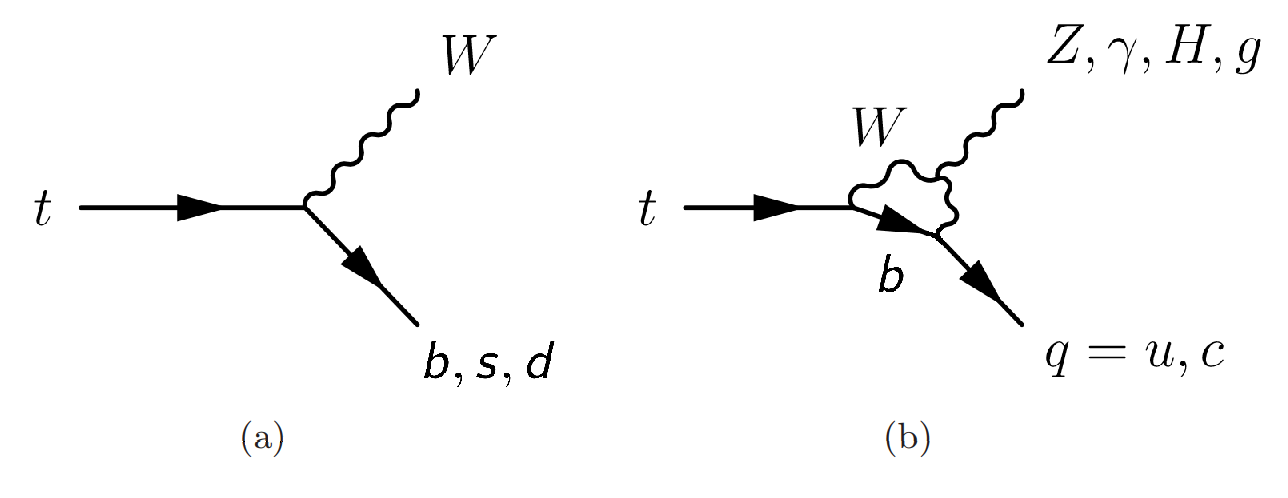
\includegraphics[width=\columnwidth]{../ThesisImages/Theory/SMTopDecays.png}
	\caption[Top quark decays in the Standard Model.]{Top quark decays in the Standard Model.}
	\label{fig:SMDecays}
\end{figure}

Since the matrix element $V_{tb}$ in the CKM matrix is essentially unity each top usually decays to a b quark and a W boson.  The final state of the top pair events are then typically categorized by the decay of the W bosons.  The W boson can decay leptonically to a lepton (electron, muon, or tau) and its associated neutrino or hadronically to quarks.  This means top pair events are described as ``all-hadronic" when both W bosons decay hadronically, ``leptonic" if both W bosons decay leptonically, or ``semi-leptonic" if one W boson decays hadronically and the other leptonically.  The ratios of these events is shown in Figure \ref{fig:ttdecayprods}.  However, because of how the tau decays and interacts, these events are typically treated separately.  Only the electron and muons are considered as the leptons in the ``semi-leptonic" final state of a $t\bar{t}$ event.  A quick counting (neglecting final state particle masses) of the final states of W bosons  is shown in Table \ref{tab:WFinals}.  The unitarity condition of the CKM matrix implies that $|V_{ud}|^2 + |V_{us}|^2 + |V_{ub}|^2 =1$.  The phase space of the final product then has 1 state for each of the leptons and approximately 3 for each of the up type quarks, so that a single top quark can be expected to decay into a lepton $\approx \frac{3}{9}$ of the time or any combination of quarks the other $\approx \frac{6}{9}$ of the time.  This holds when looking at the branching ratios of top quark pairs in Figure \ref{fig:ttdecayprods}.  The end result of this is that the regions of special interest for this dissertation, the electron and muon semi-leptonic final states, occur $\approx 30\%$ of the time.  While this is not the largest selection of the final state branching ratios the presence of a lepton makes it easier to look for these final states.

\begin{table}[]
\begin{center}
\begin{tabular}{|c|c|c|c|c|c|}
 \hline 
Decay Mode           			        & States   & Decay Mode                             &  States			   &     Decay Mode 		 	   &     States                          \\   \hline
$W^+ \rightarrow e^+ \nu_e$ 	        &1          &   $W^+ \rightarrow u\bar{d}$   &  $\times 3 |V_{ud}|^2$  &   $W^+ \rightarrow c\bar{d}$  &   $\times 3 |V_{cd}|^2$\\
$W^+ \rightarrow \mu^+ \nu_\mu$   &1          &  $W^+ \rightarrow u\bar{s}$    &  $\times 3 |V_{us}|^2$   &   $W^+ \rightarrow c\bar{s}$  &    $\times 3 |V_{cs}|^2$\\
$W^+ \rightarrow \tau^+ \nu_\tau$  &1	 &  $W^+ \rightarrow u\bar{b}$    &  $\times 3 |V_{ub}|^2$  &    $W^+ \rightarrow c\bar{b}$ &  $\times 3 |V_{cb}|^2$ \\ \hline
\end{tabular}
	\caption[Summary of final states of a W boson, when accounting for color permutations and the CKM matrix.]{Summary of final states of a $W^+$ boson, when accounting for color permutations and the CKM matrix.  The table holds true if you flip all particles to their antiparticles.}
	\label{tab:WFinals}
\end{center}
\end{table}

\begin{figure}[h!]
	\centering
	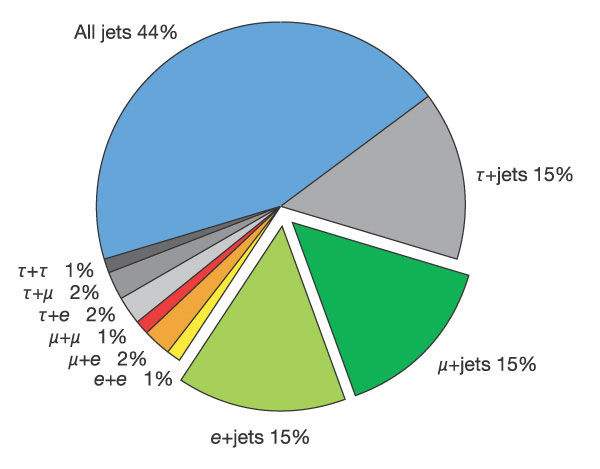
\includegraphics[width=.5\columnwidth]{../ThesisImages/Theory/topdecayproducts.jpg}
	\caption[Categorization of top quark pair decays in the Standard Model based on the decays of the W bosons.]{Categorization of top quark pair decays in the Standard Model based on the decays of the W bosons\cite{Abazov:2004cs}.}
	\label{fig:ttdecayprods}
\end{figure}


\subsection{Beyond the Standard Model Top Quark Physics}

Many questions remain open with the intricacies of the Standard Model involving top quarks.  The mass of the top quark is at a mass scale similar to the W, Z, and Higgs bosons.  Does this imply the top plays a special role in the mechanism of electroweak symmetry breaking?  After the discovery of the Higgs: why do the top quark and Higgs boson have the exact masses they do which allows the electroweak potential to be stable up to very high energy scales as well as allowing the Universe to sit in a meta-stable state\cite{TopReview}?  Because of its large mass the top quark is the main destabilizer of the Higgs potential.  It may be possible that new physics models will predict phenomena that can be more easily found in the properties of the top quark due to changes in the Higgs sector.  Many new physics models will present most dramatically in top quarks as radiative corrections to new massive particles will affect top quarks first before presenting in deviations in properties of the other, significantly lighter fermions.  For example, a new Higgs like particle would most likely couple most strongly to the top quark.  
 Now that an unprecedented number of top quarks events are accessible, the predictions of the Standard Model can be tested with much greater precision.  Top quark production modes, decay modes, couplings, and various other properties are now being measured and providing limits on the phase spaces of any new physical models that exist or ruling out entire classes of models that have yet to be written down.  Arguably the properties of top quark are one of the most likely places that will point to a new understanding of our Universe.

 %%%%%%%%%%%%%%%%%%%%%%%%%%%%%%%%%%%%%%%%%%%%%%%%

\section{The Flavor-Changing Neutral Current}
\label{sec:FCNC}
  The idea of ``flavor" in the Standard Model refers to copies of the $SU(3)_C \times U(1)_{EM}$ representation, shown previously in Table \ref{tab:SMGaugePart}.  Specifically it will be used in the discussion of the generational change of one quark into another through some interaction.  As an example, Figure \ref{fig:SMDecays}b shows a flavor changing neutral current interaction.
%%%%
\subsection{The Standard Model Flavor Sector}
Quarks that interact with $W^\pm$ bosons have interactions that stem from the kinetic term of the Standard Model Lagrangian.  If this is written out explicitly in the mass eigenstates the interaction looks like:
\[ -\frac{g}{\sqrt{2}}\begin{pmatrix} \bar{u}_L & \bar{c}_L &\bar{t}_L \end{pmatrix} \gamma^\mu W_\mu^+ V\begin{pmatrix} d_L\\s_L\\b_L\end{pmatrix}+\text{h.c.}
\]
where the W interacts directly to change the flavor of quarks from an down(up)-type to an up(down)-type quark.  The CKM matrix can be thought of as a rotation between the mass and interaction basis and the fact that the CKM matrix is non-diagonal means that the W boson interacts with quarks of different generations.  The small off-diagonal elements of the CKM matrix mean that this generational change is a significantly smaller effect than interactions that change flavors within a generation, e.g., a top quark going to a bottom quark and W boson is much more likely than a top quark decaying to a down or strange quark and a W boson.  Going two generations away from the diagonal the mixing from the CKM matrix is even smaller.  The interaction with a W boson between two quarks is the only interaction vertex in the Standard Model that allows for both flavor and generation changes.

As opposed to this flavor changing charged current interaction the FCNC is an interaction between neutral gauge bosons and fermions.  These FCNC processes involve either up or down type quarks or involve charged or neutral leptons.  The flavor of the fermion is changed but the electric charge is conserved because it interacts with a neutral boson as opposed to the $W^\pm$ like in the charged current interaction.  FCNC interactions are forbidden at tree-level in the Standard Model but can occur via higher order processes such as loops (as shown in Figure \ref{fig:SMDecays}b).

There are four neutral bosons in the Standard Model: the gluon, photon, Higgs boson, and Z boson.  Each of these can mediate FCNC interactions but all are forbidden at tree-level.  The gluon and photon correspond to exact gauge symmetries and have diagonal, flavor universal couplings since their interactions with fermions come through the kinetic terms.  The ramification of this is that they only interact with fermions of the same flavor.  The Standard Model Higgs cannot couple to fermions of different flavor since the Standard Model fermions are chiral and the Higgs couplings to fermions align with the fermion mass matrix.  In the Standard Model there is only a single Higgs doublet and the only source of the fermionic masses is the Higgs vacuum expectation value.  The Z boson can only connect to quarks from the same type (up or down).  When you move from the interaction to the mass eigenstates the rotation matricies only include terms such as $U_{uL}U_{uL}^\dagger = 1$ as opposed to the CKM matrix terms ($U_{uL}U_{dL}^\dagger$) which means these couplings are also flavor universal. 
The Standard Model FCNC suppression is built in through these means as opposed to generation-changing charged current processes.  The charged current processes rely on the CKM parameters which are free parameters of the Standard Model and as such are measured and ``put in."  These FCNCs are suppressed multiple ways in the Standard Model.

\subsection{The GIM Mechanism}
Historically the original Cabibbo model of particle physics only had three quarks: the up, down, and strange.  Studies of Kaon decay during the late 1960's suggested there were no neutral current interactions in the Standard Model at the time.  The decay $K^+ \rightarrow \mu^+ \nu_\mu$ was observed but the process $K_L^0 \rightarrow \mu^+ \mu^- $ which was predicted was not observed.  Even in the absence of a tree level decay the $K_L^0$ decay was still predicted via a box diagram through the exchange of W bosons shown in Figure \ref{fig:KaonBox}.

\begin{figure}[h!]
	\centering
	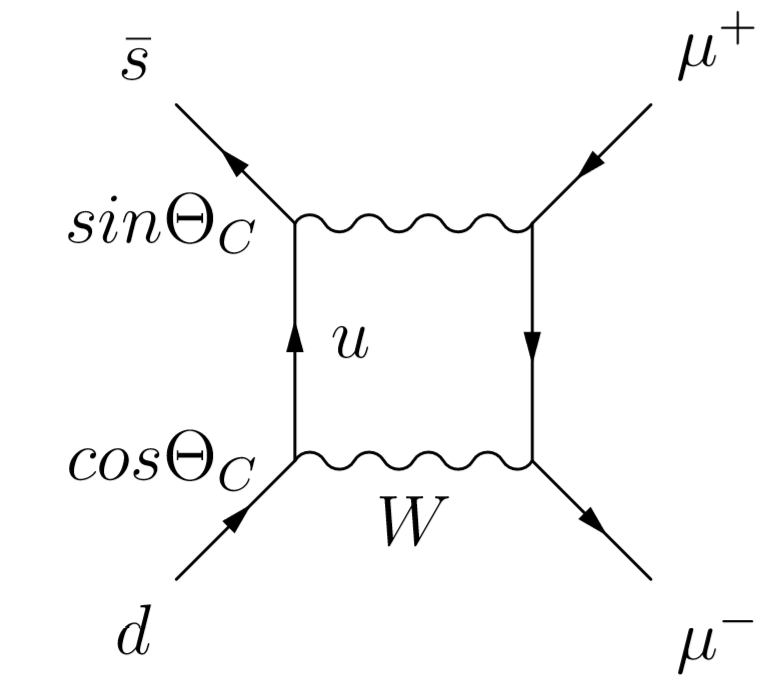
\includegraphics[width=.4\columnwidth]{../ThesisImages/Theory/GIMDiagramsa.png}
	\caption{Box diagram of $K_L^0 \rightarrow \mu^+ \mu^-$ through the exchange of W bosons.}
	\label{fig:KaonBox}
\end{figure}

Interactions at the time were thought to have strangeness quantum number interactions that changed strangeness in the following way:
\[ \Delta S=0 : u\bar{u} +d\bar{d}\text{cos}^2\Theta_C + s\bar{s} \text{sin}^2\Theta_C \]\[
\Delta S =1: (s\bar{d} + d\bar{s})\text{sin}\Theta_C \text{cos}\Theta_C  \]

The non-observation of the predicted decay led Glashow, Iliopoulous, and Maiani to predict the existence of a fourth quark, the charm, in 1970\cite{GIM}.  The addition of the charm led to two quark doublets and an almost perfect cancellation between the box diagrams:

\begin{figure}[h!]
	\centering
	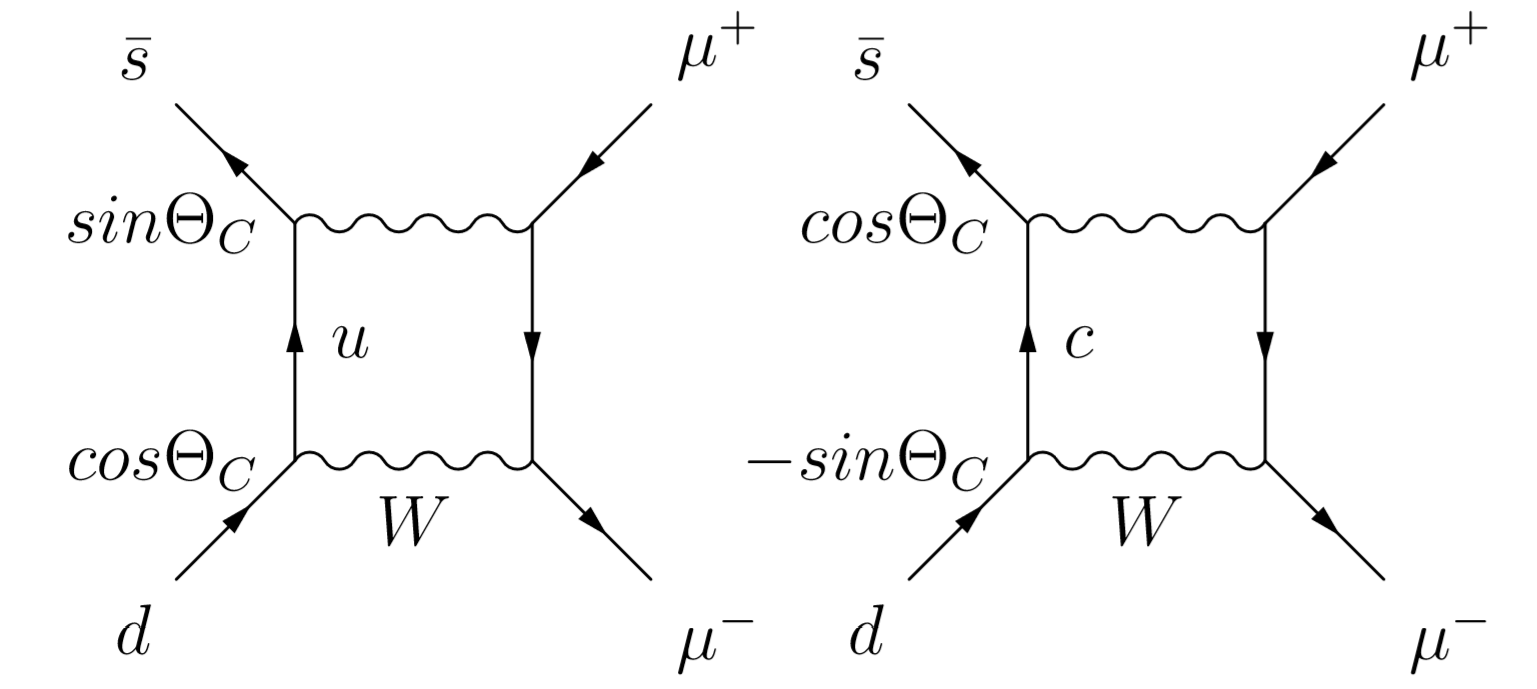
\includegraphics[width=.9\columnwidth]{../ThesisImages/Theory/GIMDiagrams.png}
	\caption{Box diagrams of $K_L^0 \rightarrow \mu^+ \mu^-$ through the exchange of W bosons after the inclusion of the charm quark.}
	\label{fig:KaonBox2}
\end{figure}

These box diagrams mean that the strangeness change in interactions can be rewritten as 
\[ \Delta S=0 : u\bar{u} + c\bar{c} +(d\bar{d}+s\bar{s})\text{cos}^2\Theta_C + (s\bar{s}+d\bar{d}) \text{sin}^2\Theta_C \]\[
\Delta S =1: (s\bar{d} + d\bar{s} -d\bar{s}-s\bar{d})\text{sin}\Theta_C \text{cos}\Theta_C  \]

The addition of the charm means that, in the approximation $m_c = m_u$, the $\Delta S =1$ terms cancel exactly, as the new box diagrams show in Figure \ref{fig:KaonBox2}.  The FCNC interactions in top quark decays are suppressed through this mechanism as well, with the further inclusion of the bottom and top quarks.  They are further suppressed by being proportional to the quark mixing of off-diagonal elements in the CKM matrix, which are significantly less than 1.  A loop diagram for top quark FCNC is shown in Figure \ref{fig:FCNCLoop}.  This loop process is very rare.  The Standard Model branching ratio for these top FCNC interactions is shown along predicted enhancements from a variety of models of physics beyond the Standard Model in Table \ref{tab:FCNCLimits}.

\begin{figure}[h!]
	\centering
	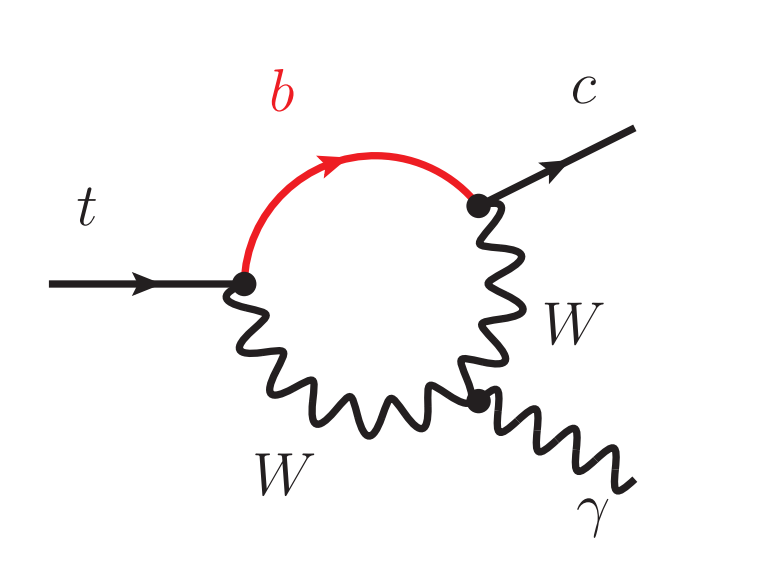
\includegraphics[width=.5\columnwidth]{../ThesisImages/Theory/FCNCLoop.png}
	\caption{An example loop diagram of a top quark decaying to a light quark and a photon.}
	\label{fig:FCNCLoop}
\end{figure}


\begin{table}[]
\begin{center}
\begin{tabular}{lllllll}
 \hhline{=======}
Process                                    & SM                        & 2HDM                   & QS                           & MSSM                   & RPV                          & XD                                 \\   \hline 
$t\rightarrow u\gamma $ &    $ 4*10^{-16} $        & $ -  $                   & $ \leq 4*10^{-8} $   & $ \leq 10^{-8} $ & $ \leq 10^{-9} $      &  $- $                                             \\
$t\rightarrow c\gamma $ &    $ 5*10^{-14} $        & $ \leq 10^{-7}   $ & $ \leq 4*10^{-8} $ & $ \leq 10^{-8} $ & $ \leq 10^{-9} $     & $ \leq 10^{-9}  $\\ \hline
$t\rightarrow u Z                    $ & $ 7*10^{-17} $  & $ -                     $ & $ \leq 6*10^{-4} $ & $ \leq 10^{-7} $ & $ \leq 10^{-6} $     & $ -  $                                             \\
$t\rightarrow c Z                    $ & $ 1*10^{-14} $  & $ \leq 10^{-6}   $ & $ \leq 6*10^{-4} $ & $ \leq 10^{-7} $ & $ \leq 10^{-6} $     & $ \leq 10^{-5} $ \\
$t\rightarrow u g                    $ & $ 4*10^{-14} $  & $ -                     $ & $ \leq 9*10^{-7} $ & $ \leq 10^{-7} $ & $ \leq 10^{-6} $     & $ -  $                                             \\
$t\rightarrow c g                    $ & $ 5*10^{-12} $  & $ \leq 10^{-4}   $  & $ \leq 9*10^{-7} $ & $ \leq 10^{-7} $ & $ \leq 10^{-6} $    & $ \leq 10^{-10} $ \\
$t\rightarrow u H                    $ & $ 2*10^{-17} $  & $ \leq 6*10^{-6} $ & $ -                      $ & $ \leq 10^{-5} $ & $ \leq 10^{-9} $     & $ -    $                                           \\
$t\rightarrow c H                    $ & $ 3*10^{-15} $  & $ \leq 2*10^{-3} $ & $ -                      $ & $ \leq 10^{-5} $ & $ \leq 10^{-9} $     & $ \leq 10^{-4} $ \\
\hhline{=======}
\end{tabular}
	\caption[Expected branching ratios for various flavor changing neutral current processes in the Standard Model and multiple theories that predict enhancements to the branching ratio.  Two-Higgs Double Models with flavor-violating Yukawa couplings (2HDM), quark single models (QS), minimal supersymmetry models with 1TeV squarks and gluinos (MSSM), R-parity violating supersymmetry models (RPV), and extra-dimensional models (XD).]{Expected branching ratios for various flavor changing neutral current processes in the Standard Model\cite{2HDM-2} and multiple theories that predict enhancements to the branching ratio.  Two-Higgs Double Models with flavor-violating Yukawa couplings (2HDM) \cite{2HDM-2,2HDM-3}, quark single models (QS) \cite{QS-1,QS-2}, minimal supersymmetry models with 1TeV squarks and gluinos (MSSM) \cite{MSSM}, R-parity violating supersymmetry models (RPV) \cite{RPVSusyFCNC}, and extra-dimensional models (XD) \cite{XDFCNC}.}
	\label{tab:FCNCLimits}
\end{center}
\end{table}

\subsection{New Physics With Enhancements to FCNCs}
\label{sec:bsmFCNC}
Various theoretical models that include physics beyond what is included in the Standard Model are proposed to solve problems that exist with the Standard Model or an explanation of known phenomena that are not in agreement with the Standard Model.  Various models seek to solve different problems, e.g., providing a dark matter candidate or fixing the naturalness problem of the Standard Model resulting from an unexpectedly high amount of fine-tuning from loop corrections to the Higgs mass.  
Top quark FCNCs in the Standard Model are currently so far from experimental reach ($\approx 10$ orders of magnitude) that they are impossible to observe even with major improvements to the accelerator and detector techonologies.  Table \ref{tab:FCNCLimits} also shows a variety of theories beyond the Standard Model which predict large enhancements to FCNC top couplings.  For the most part these enhancements come from terms that have very heavy particles moving in the loops.  Therefore searching for FCNCs with top quarks provides a particularly good handle to search for evidence of, or to rule out, models of new physics by lowering the expected limit.  An explanation of the various models explored in Table \ref{tab:FCNCLimits} follows.

\textbf{Two-Higgs-Doublet Models (2HDM): } 2HDM are a simple extension of the Standard Model which contain two Higgs doublets instead of the one currently contained in the Standard Model.  This leads to a much richer phenomenology in the Higgs sector with two CP even neutral Higgs bosons ($h$ and a heavier $H$), a CP odd pseudoscalar $A$, and two charged Higgs bosons $H^\pm$.  The currently discovered Higgs boson can be mapped to either h or H depending on various limits in the model of choice.  These models can typically be described by an additional six parameters: the four Higgs masses ($m_h, m_H,m_A,m_{H^\pm}$), the ratio of the two vacuum expectation values and a mixing angle that diagonalizes the mass matrix of the neutral CP even Higgs bosons.  Many supersymmetric models predict the existence of an extra Higgs doublet.  Some of these models also attempt to explain the baryon asymmetry of the Universe\cite{Trodden:1998ym}.
2HDM Models predict very large enhancements to FCNC interactions due to an extension of the electroweak symmetry breaking sectors.  Some of these models (type III 2HDM, and models of minimal flavor violation) include tree level FCNCs\cite{Branco:2011iw} which is why the enhancement brings the branching ratio up to an observable level.

\textbf{Quark Singlet Models (QS): } QS involve an extension to the Standard Model in the form of an extra vector-like quark singlet that couples strongly to the top quark, typically in the form of a top-partner quark.  These heavier $t'$ quarks could explain the fine-tuning of the Higgs boson mass through cancellation of some or all of the top loop diagrams present in the radiative corrections to the Higgs mass.  These models generally imply then that the CKM matrix is no longer unitary and tree level FCNCs are allowed which offers a great enhancement to potential branching ratios\cite{QS-1,QS-2}.

\textbf{Minimal Supersymmetric Models (MSSM): }  Supersymmetric models where every Standard Model particle has a super particle partner typically aim to solve multiple problems with the Standard Model at once.  In general the lightest supersymmetric particle, which is stable, provides a good dark matter candidate.  MSSM models have super partner quarks (squarks) and super partner gluons (gluinos) on a mass scale of $\approx 1 \text{ TeV}$.  Top FCNCs can occur through loop diagrams still, as they do in the Standard Model, but the loop is enhanced as it includes the supersymmetric particle of the top quark (the heavier stop quark)\cite{MSSM, MSSM-2}.

\textbf{R-Parity Violating Supersymmetric Models (RPV): }  Another supersymmetric model R parity is no longer conserved because all superpartners are odd under the parity.  FCNCs can also occur at the one loop level in these models in loops which no longer conserve baryon or lepton number\cite{RPVSusyFCNC}.

\textbf{Extra-dimensional Models (XD): }  XD Models are Randall-Sundrum models that describe the Universe as a warped-geometry higher dimensional space where elementary particles are localized on a (3+1)-dimensional brane.  These models offer a potential solution to the hierarchy problem of the Standard Model by adding in a mechanism to explain the difference between the typical scales over which FCNCs take place (the electroweak scale) and the Planck scale.  In these models FCNCs exist due to flavor-violating couplings between Standard Model fermions and Kaluza-Klein excitations of the gauge bosons in the Standard Model\cite{XDFCNC}.  Due to their overlap in the extra dimension with Kaluza-Klein guage modes the flavor-violating couplings will be largest in the top sector.


\subsection{Current Measurements of Top FCNCs}

All four of the neutral boson mediated FCNC channels can be searched for individually and model independently.  Each channel will have its own signature and various advantages and disadvantages in performing the search.  Each of the potential tree-level diagrams is shown in Figure \ref{fig:AllFCNCs}, all of which are forbidden at tree level in the Standard Model.  %%%%%%%%%%%%%%%%
\begin{figure}[h!]
	\centering
	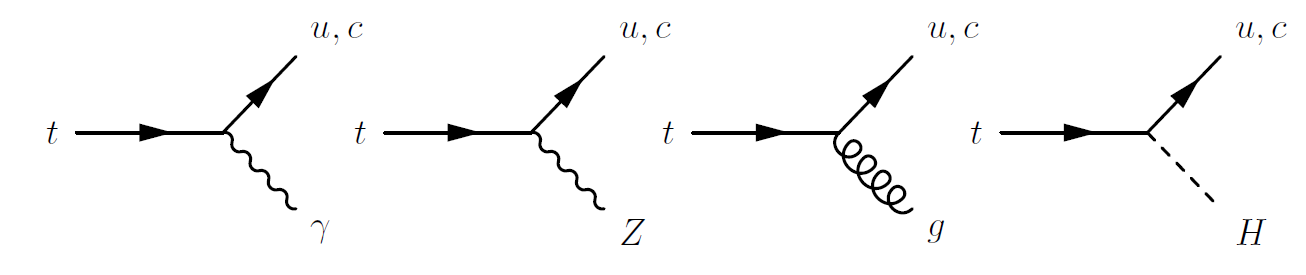
\includegraphics[width=\columnwidth]{../ThesisImages/Theory/AllFCNCDiagrams.png}
	\caption{Flavor changing neutral current top quark decays.}
	\label{fig:AllFCNCs}
\end{figure}

The FCNC channels involving all of the various neutral bosons can be searched for with the ATLAS detector in both single-top production modes as well as the decay mode through $t\bar{t}$ events.  All of the production channels provide a sharp separation between $u\rightarrow tX$ and $c\rightarrow tX$ but have fewer events than searching in the decay mode using $t\bar{t}$ events.  Some final states of these various FCNC events such as those involving the decay mode search for $t\rightarrow q Z$ exploit the tri-lepton final state ($Z\rightarrow ll$, with the other top decaying leptonically $t\rightarrow bW\rightarrow bl\nu$).  The FCNC process involving the Higgs boson has the advantage of being able to look in a wide range of potential final states of the Higgs and can be successfully tackled using a variety of different methods.

\begin{figure}[h!]
	\centering
	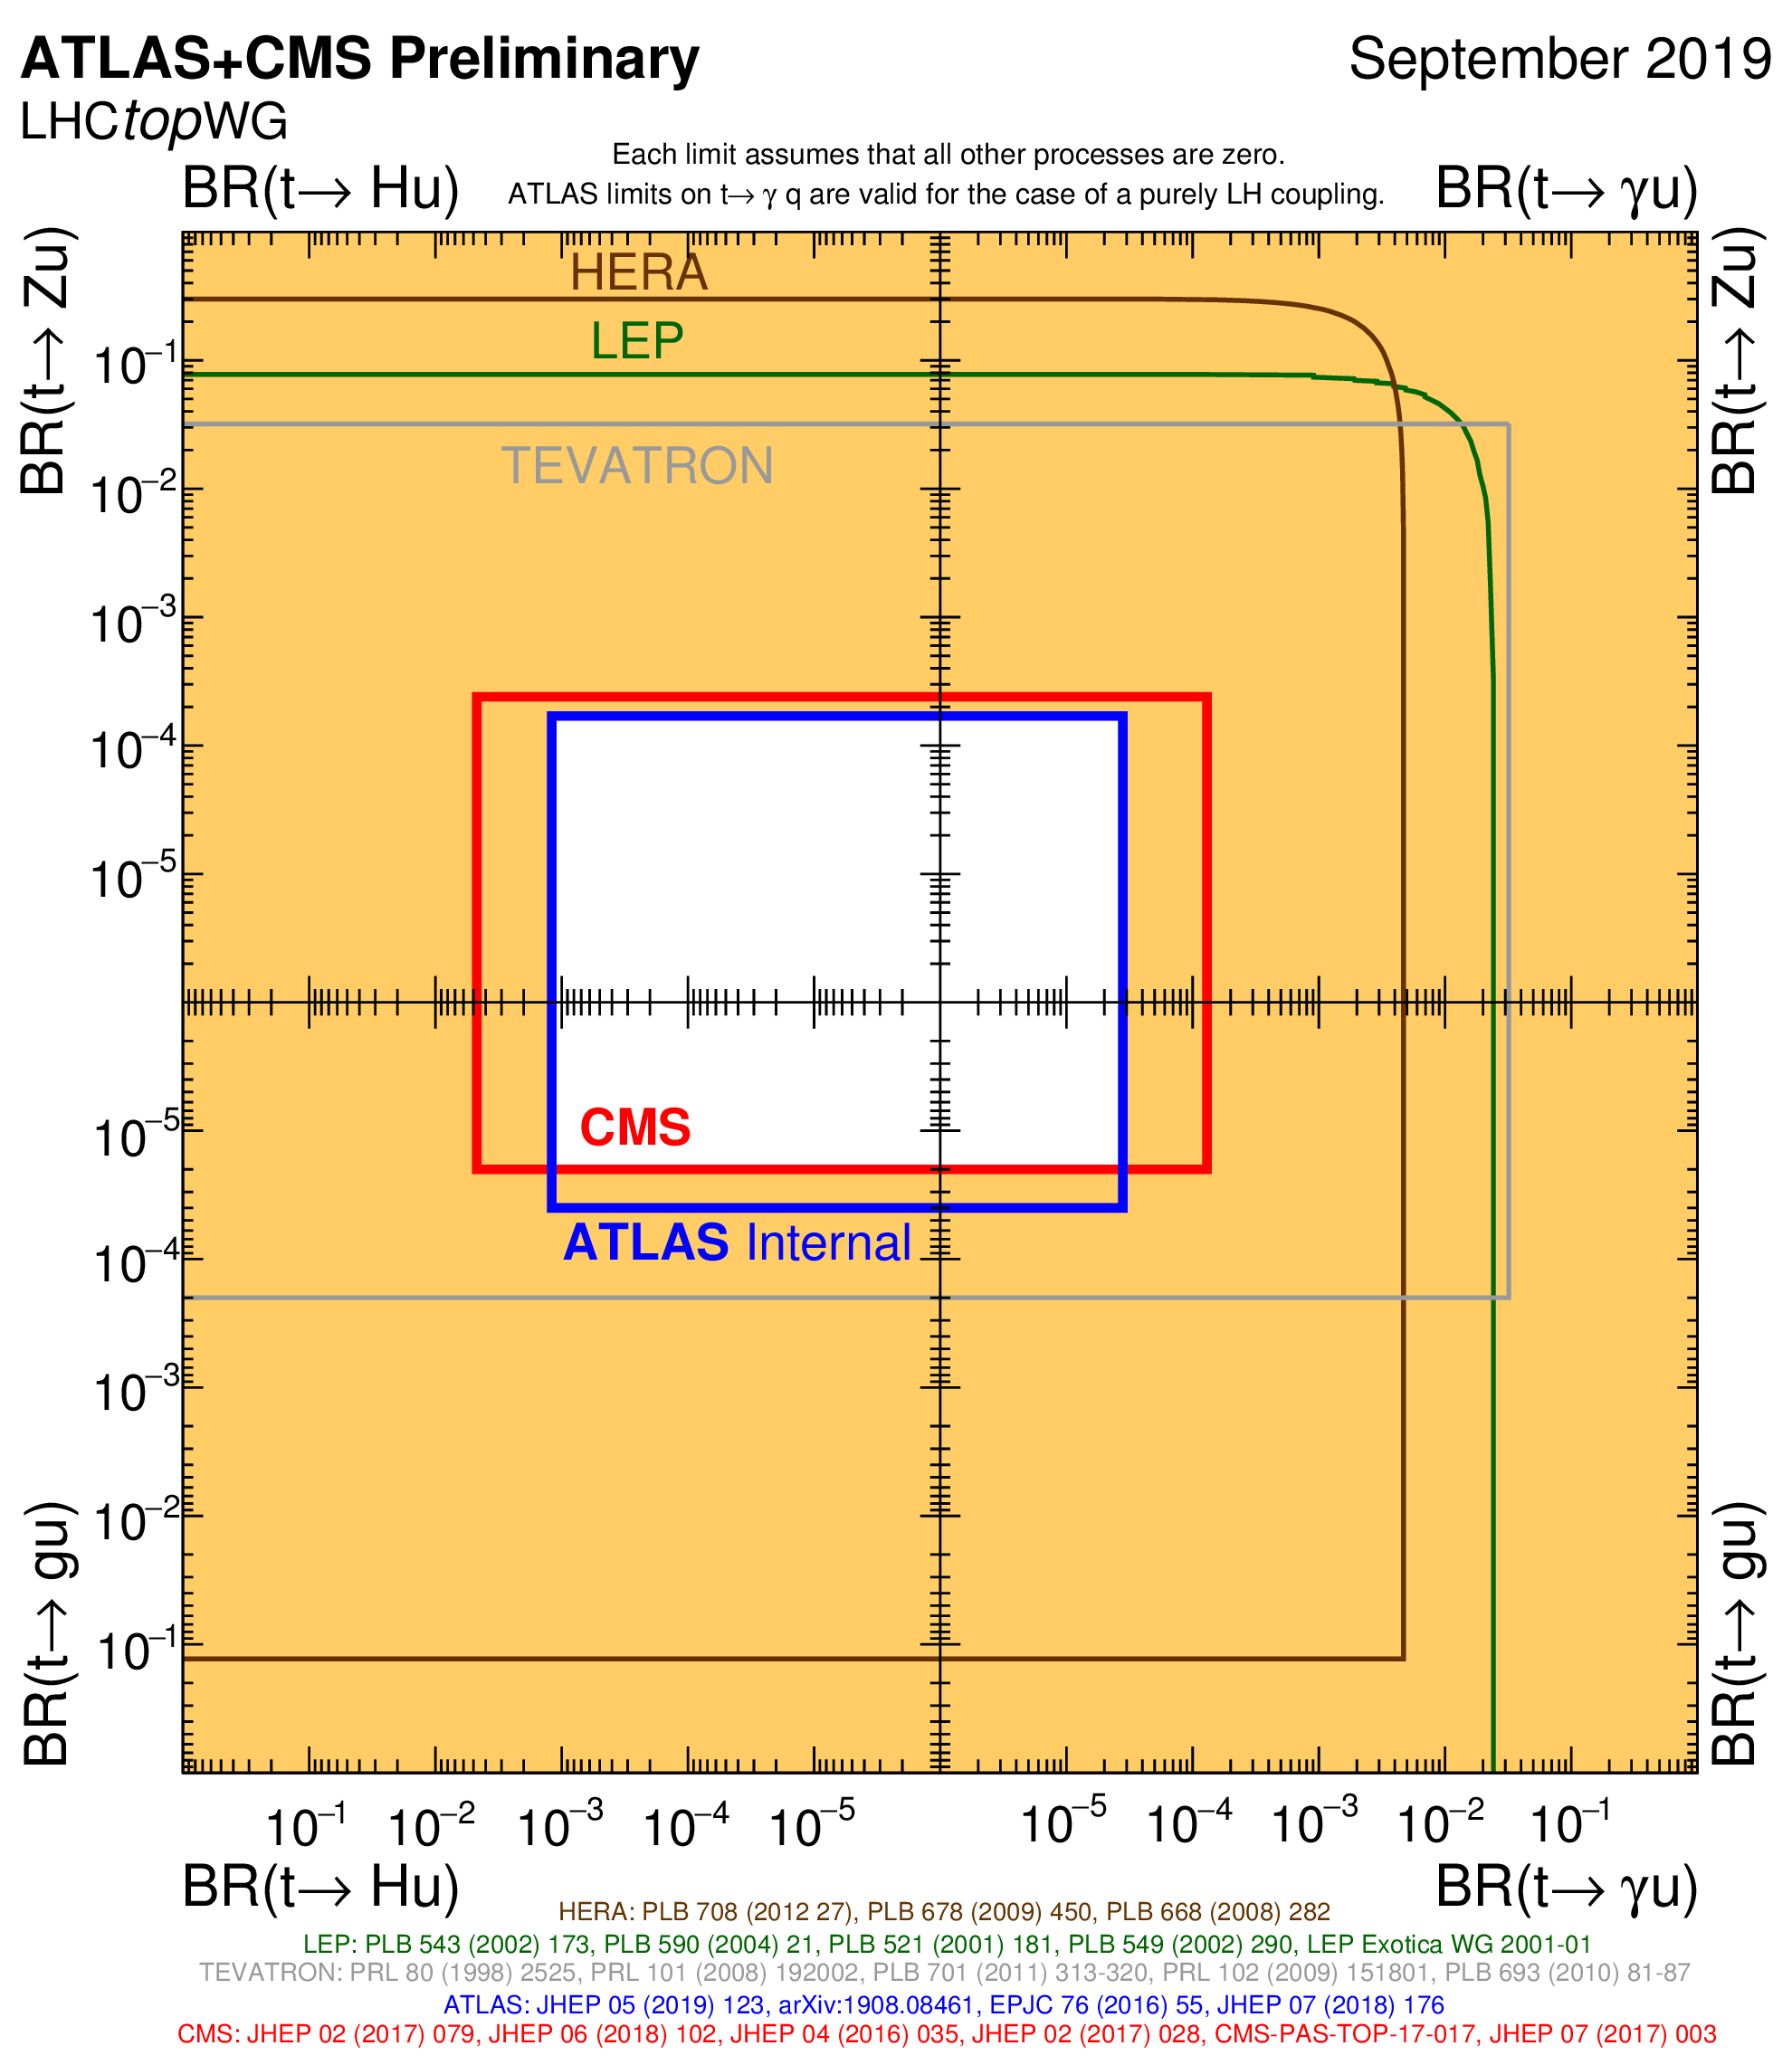
\includegraphics[width=.5\columnwidth]{../ThesisImages/Theory/fcnc_tXu_sep18.png}
	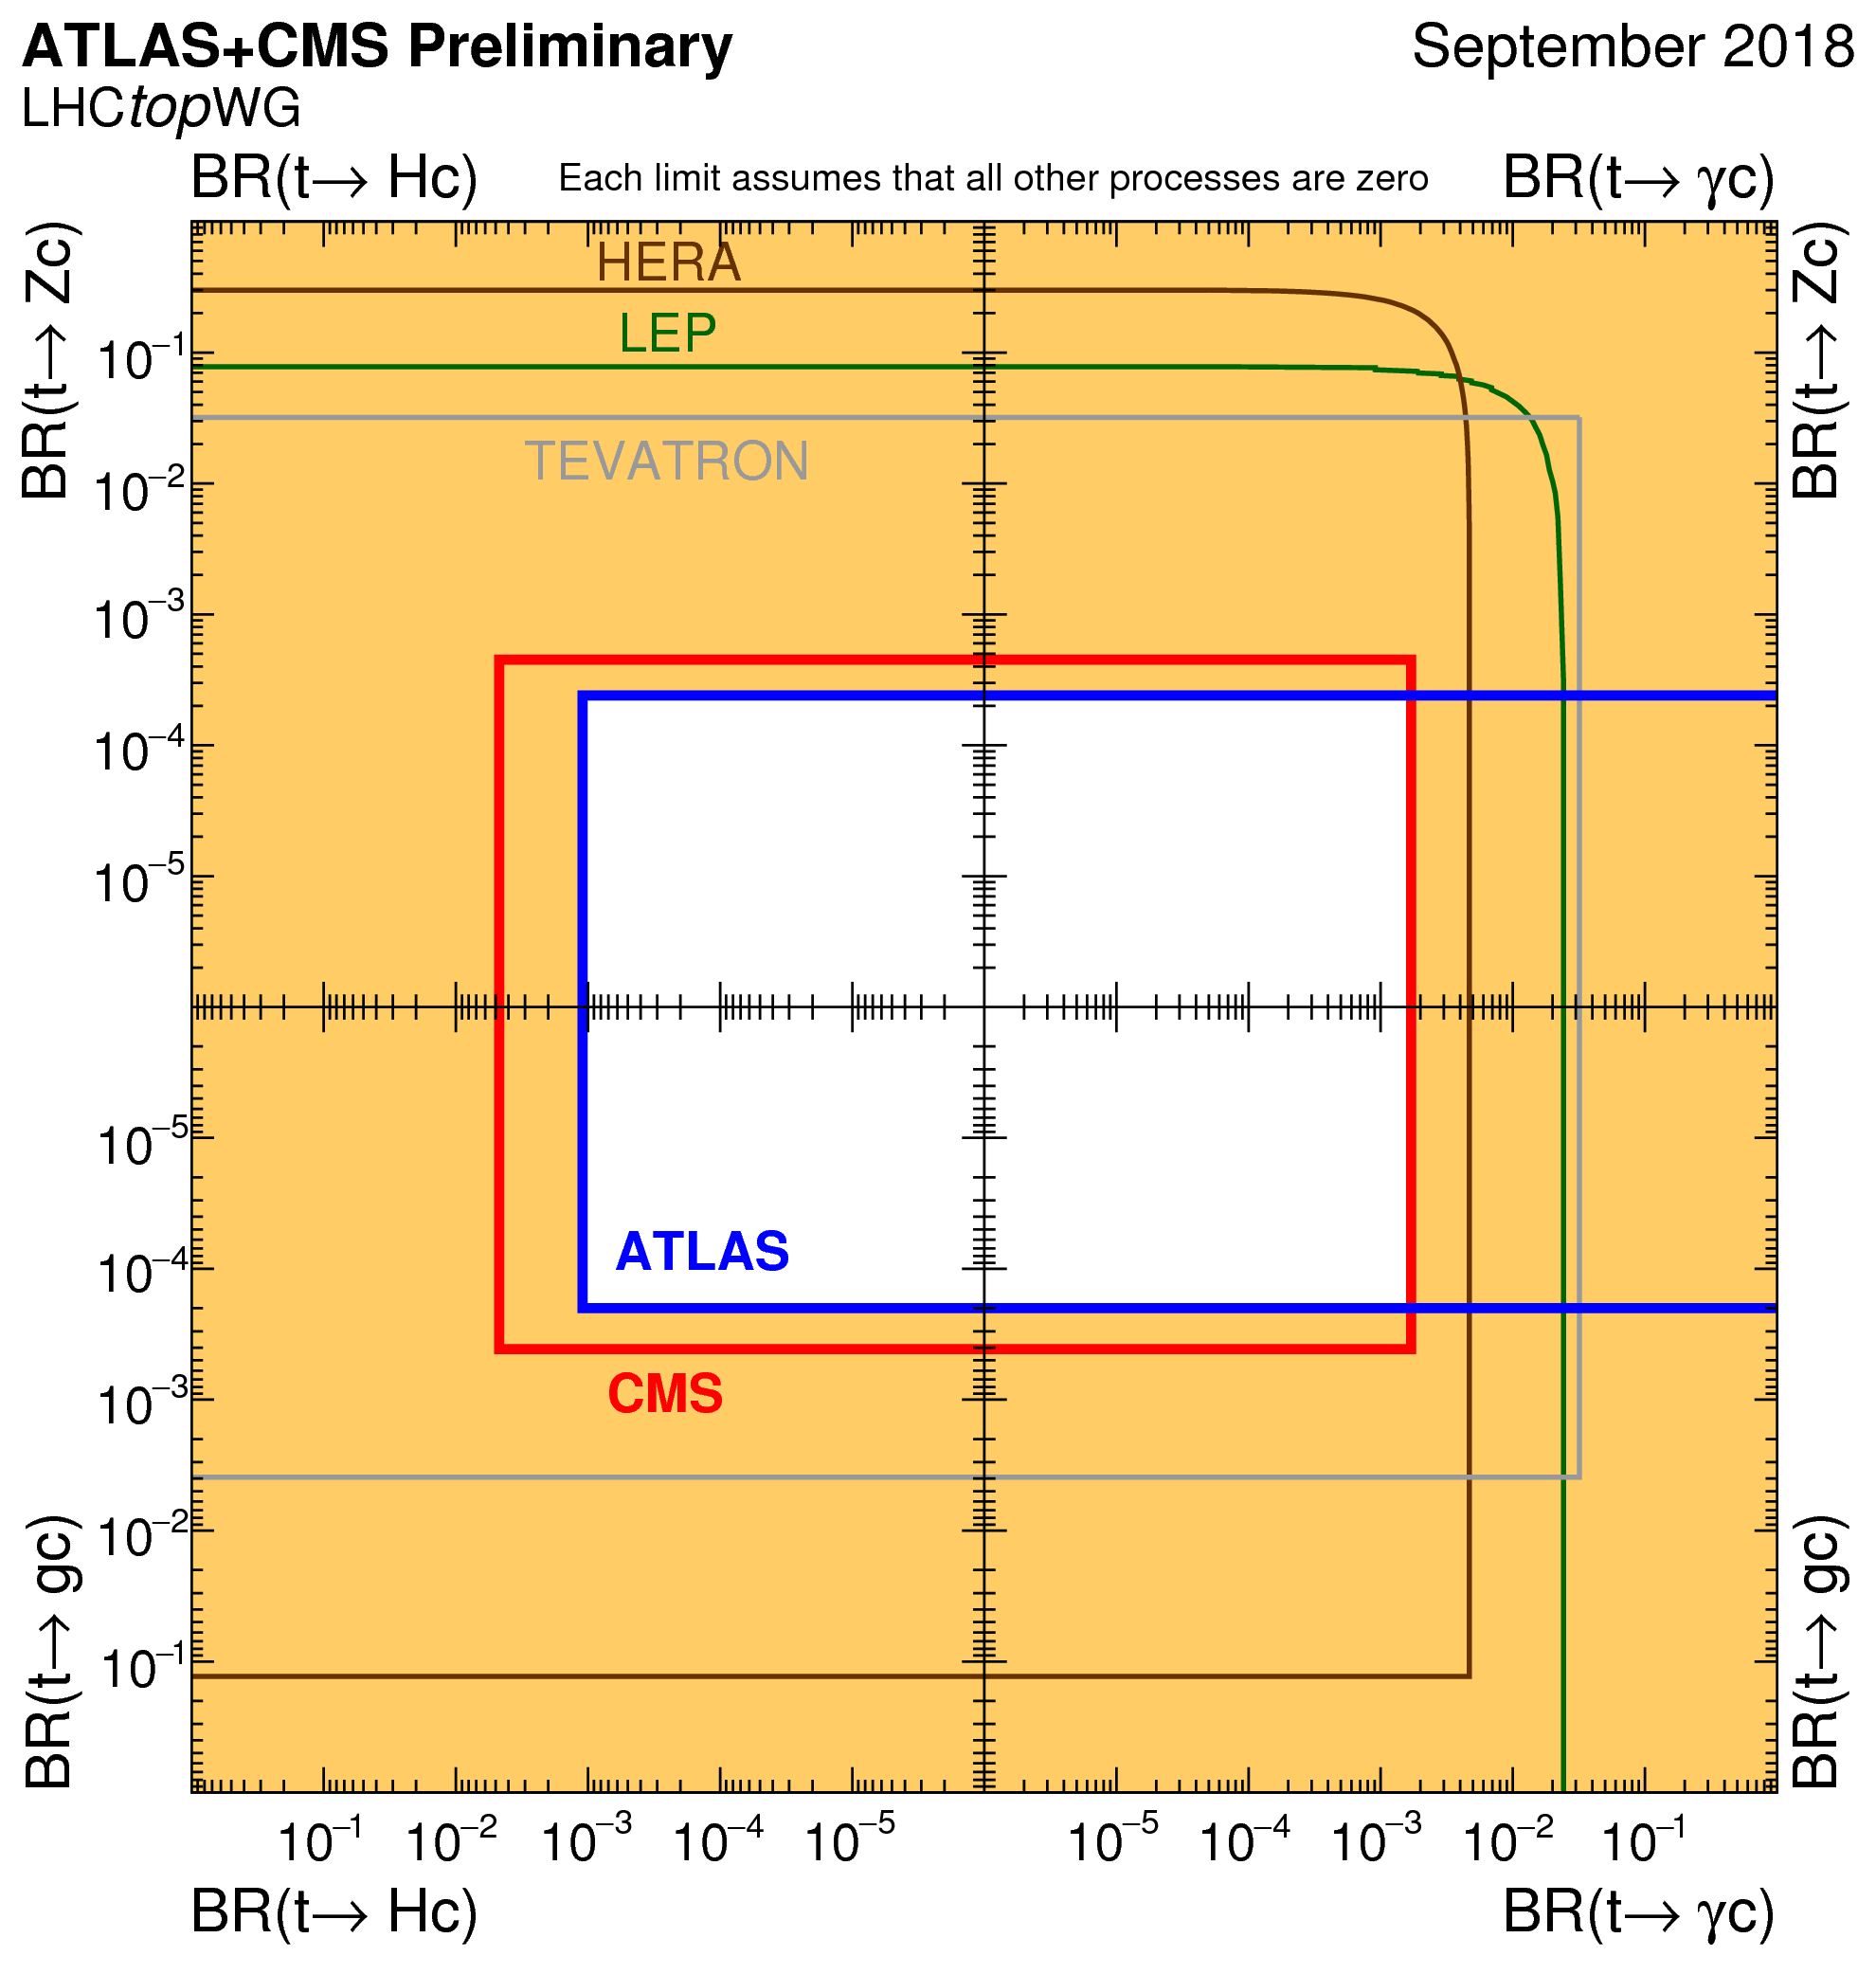
\includegraphics[width=.5\columnwidth]{../ThesisImages/Theory/fcnc_tXc_sep18.png}
	\caption[Flavor changing neutral current limits from a variety of expeiments in every channel $t\rightarrow uX$(top) and $t\rightarrow cX$(bottom).]{Flavor changing neutral current limits from a variety of expeiments in every channel $t\rightarrow uX$(top) and $t\rightarrow cX$(bottom) \cite{TopWG}.  The blue box shows the current ATLAS limits on the FCNC processes, the vertical lines show the Higgs and $\gamma$ limits while the horizontal lines show the Z and g limits.}
	\label{fig:FCNCLimsBox}
\end{figure}

Limits have been set on these FCNC processes at various experiments in the past.  The electron-proton collider HERA at DESY, the electron-proton collider LEP at CERN, and the proton-proton colliders the Tevatron at Fermilab and the LHC at CERN have all had experiments searching for the FCNC proccesses.  The collected limits of these experiments are shown in Figure \ref{fig:FCNCLimsBox}.  Due to the energy of these early colliders 209 GeV center of mass energy for LEP and 318 GeV for HERA only production modes could be searched for as they are below the production threshold for $t\bar{t}$ pairs. The diagrams searched for at these experiments are shown in Figure \ref{fig:fcncHera} (HERA) and Figure \ref{fig:fcncLep} (LEP).
\begin{figure}[h!]
	\centering
	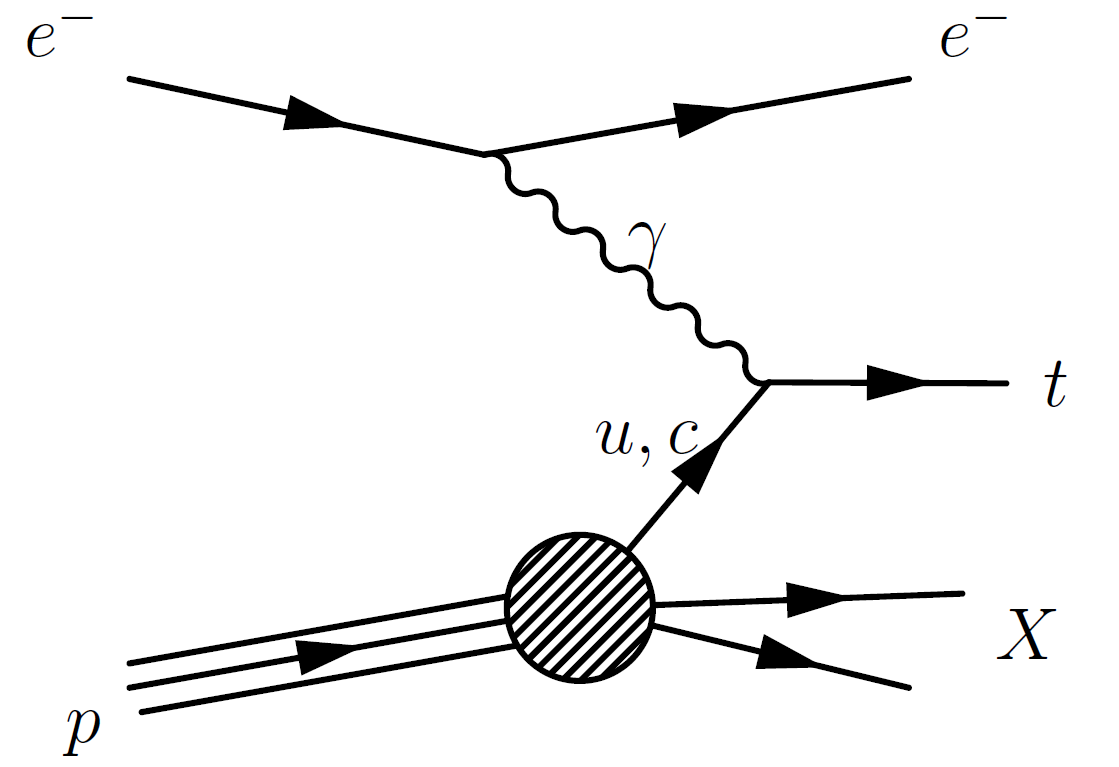
\includegraphics[width=.4\columnwidth]{../ThesisImages/Theory/HeraFCNC.png}
	\caption{FCNC diagram for the search in single top production at the electron-proton collider HERA.}
	\label{fig:fcncHera}
\end{figure}
\begin{figure}[h!]
	\centering
	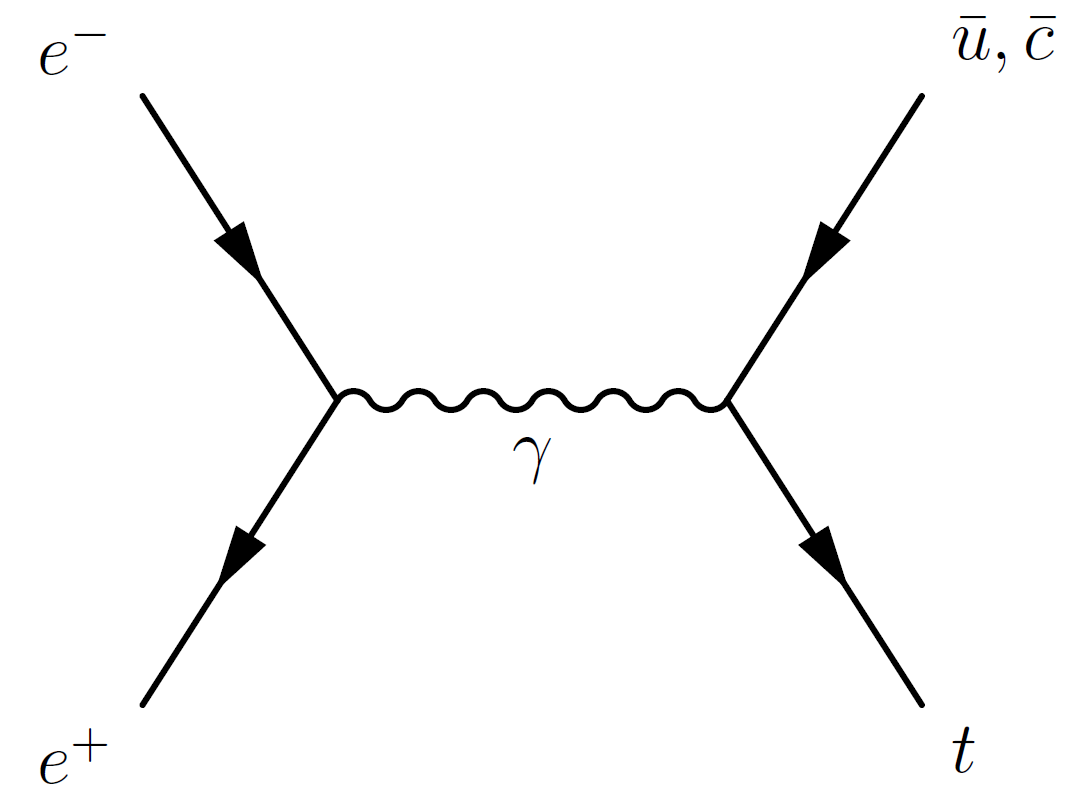
\includegraphics[width=.4\columnwidth]{../ThesisImages/Theory/LepFCNC.png}
	\caption{FCNC diagram for the search in single top production at the electron-positron collider, LEP.}
	\label{fig:fcncLep}
\end{figure}

\begin{figure}[h!]
	\centering
	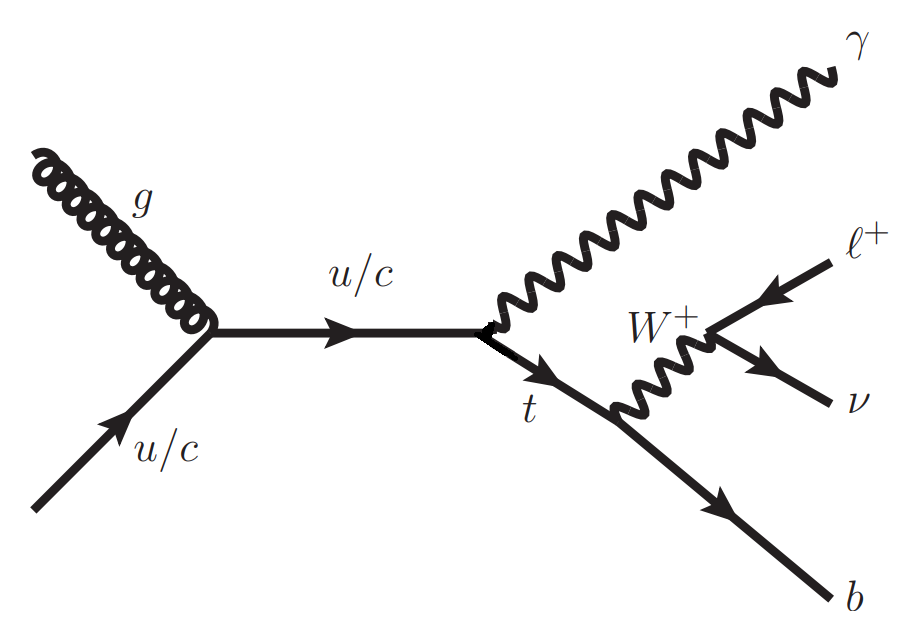
\includegraphics[width=.4\columnwidth]{../ThesisImages/Theory/ProductionMode.png}
	\caption[FCNC diagram for the search in single top production with the ATLAS detector.]{FCNC diagram for the search in single top production with the ATLAS detector\cite{GregorFCNC}. }
	\label{fig:ProductionMode}
\end{figure}

Shown in Figure \ref{fig:FCNClimits} are the Standard Model theoretical predictions, various beyond the Standard Model predictions (as discussed in Section \ref{sec:bsmFCNC}), and experimental limits for all processes $t\rightarrow Xq$ where q is an up-type quark and X is any neutral boson.  
\begin{figure}[h!]
	\centering
	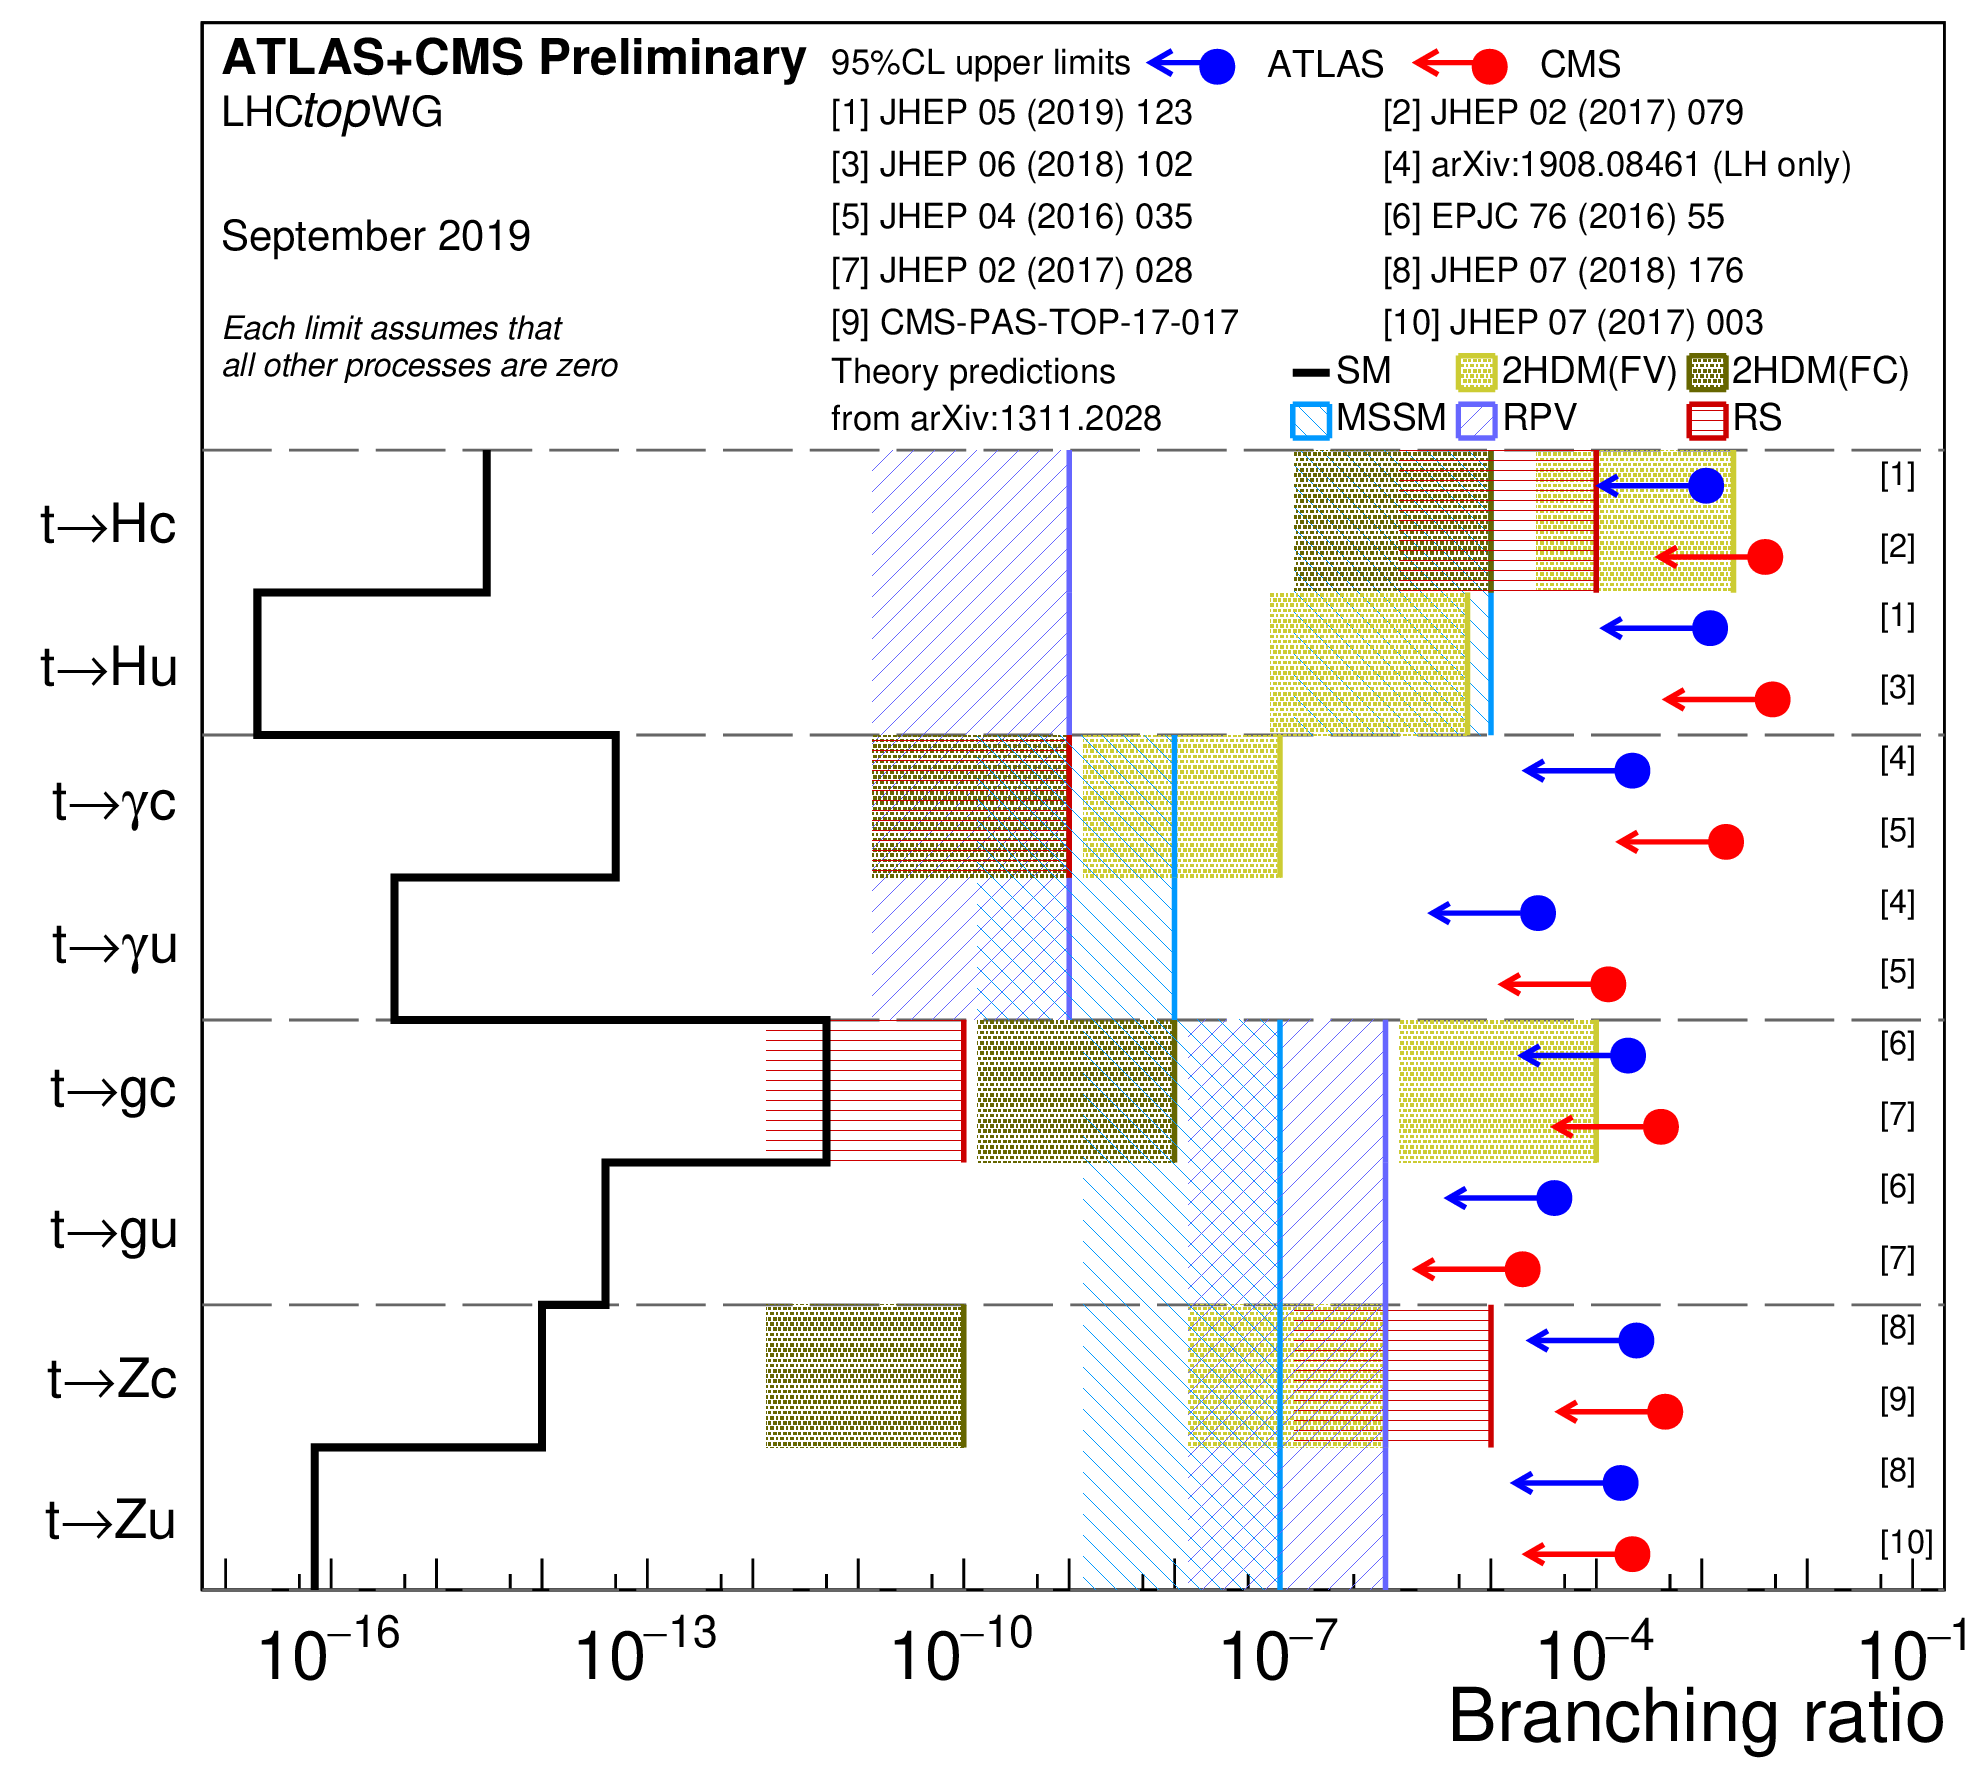
\includegraphics[width=.8\columnwidth]{../ThesisImages/Theory/AllFCNCLimits.png}
	\caption[Flavor changing neutral current theoretical branching ratios and experimental limits (both ATLAS and CMS) updated through 2018. ]{Flavor changing neutral current theoretical branching ratios and experimental limits (both ATLAS and CMS) updated through 2018 \cite{TopWG}. }
	\label{fig:FCNClimits}
\end{figure}


Figure \ref{fig:FCNClimits} shows the current published results for all top quark FCNC searches.  The most recent ATLAS detector result is the production mode search of the $t\rightarrow q\gamma$ vertex, the Feynman diagram shown in Figure \ref{fig:ProductionMode}, using 81 $\text{fb}^{-1}$ of data (LHC data runs between 2015-2017).  Upper limits have been set on $t\rightarrow u \gamma$ left-handed (right-handed) branching ratio of $2.8\times 10^{-5}$ ($6.1\times 10^{-5}$) and upper limits on $t \rightarrow c \gamma$ left-handed (right-handed) branching ratio of $22\times10^{-5}$ ($18\times10^{-5}$) \cite{GregorFCNC}.  Production mode searches offer better reach for $t\rightarrow u \gamma$ over $t\rightarrow c \gamma$ due to the higher prevelance of up quarks in the parton distribution function of the colliding protons.

This dissertation presents a search for the process $t\rightarrow q \gamma$ in the decay channel using top quark pair events.  The process $t\bar{t} \rightarrow bWq\gamma \rightarrow bl\nu q\gamma$ will be searched for using the ATLAS detector.  This final state ($b l \nu q \gamma$) is a straightforward channel in that it has one of each type of object that can be reconstructed with ATLAS.  There are 2 jets from the quarks but one is a b-jet that has qualities that can distinguish it from a normal quark jet which will be discussed in Section \ref{sec:bjetReco}.  In addition to the jets the final state also has a charged lepton (an electron or muon), a photon, and a neutrino.  The reconstruction of these objects is discussed in Chapter \ref{ch:Simulation}.  The FCNC process is a unique process where a top quark decays directly into an up-type quark and a photon.  The jet and photon we measure are required to be reconstructed into a top quark by measuring the invariant mass requirement which gives an excellent handle for separating signal from background.






%
%CKM Matrix\cite{PDG2018}:
%\[
%\begin{pmatrix}
%d' \\ s' \\ b'
%\end{pmatrix}
%=
%\begin{pmatrix}
%V_{ud} & V_{us} & V_{ub} \\
%V_{cd} & V_{cs} & V_{cb} \\
%V_{td} & V_{ts} & V_{tb} 
%\end{pmatrix}
%= 
%\begin{pmatrix}
%d \\ s \\ b
%\end{pmatrix}
%\]

%
%%%%%%%%%%%%%%%%%%%%%%%%%%%%%%%%%%%%%%%%%%%%%%%
%%%%%%%%%%%%                                                                                                   %%%%%%%% 
%%%%%%%%%%%%                           BEN                                                                  %%%%%%%% 
%%%%%%%%%%%%                                                                                                   %%%%%%%% 
%%%%%%%%%%%%%%%%%%%%%%%%%%%%%%%%%%%%%%%%%%%%%%%

%\begin{figure}[]
%	\centering
%	\subfloat[]{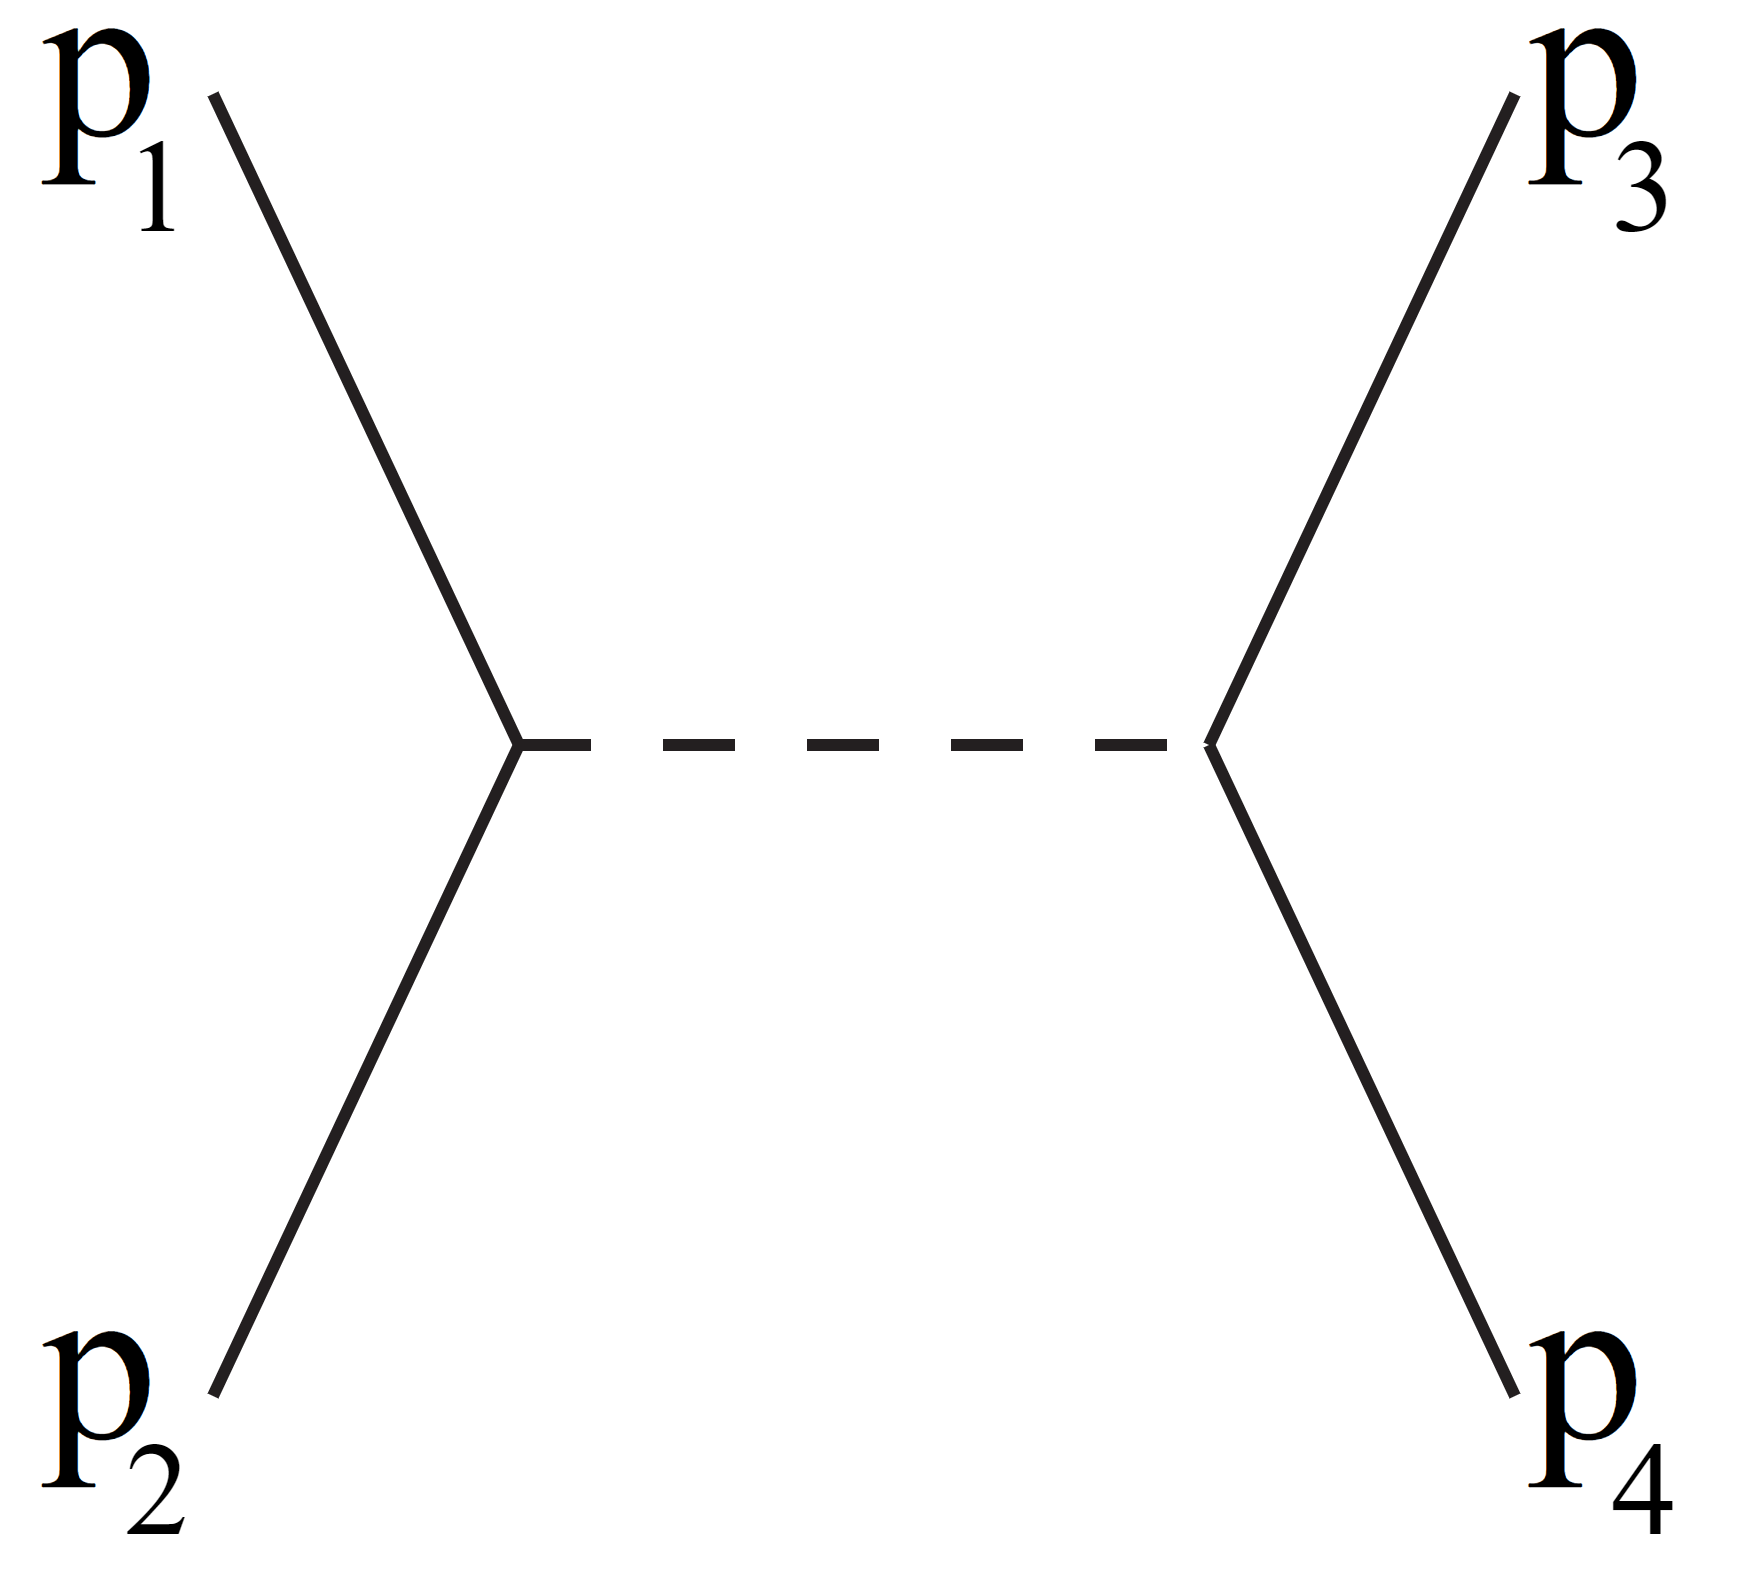
\includegraphics[width=0.35\columnwidth]{figures/Theory/SChannel.png}}
%	\hspace{0.1\columnwidth}%
%	\subfloat[]{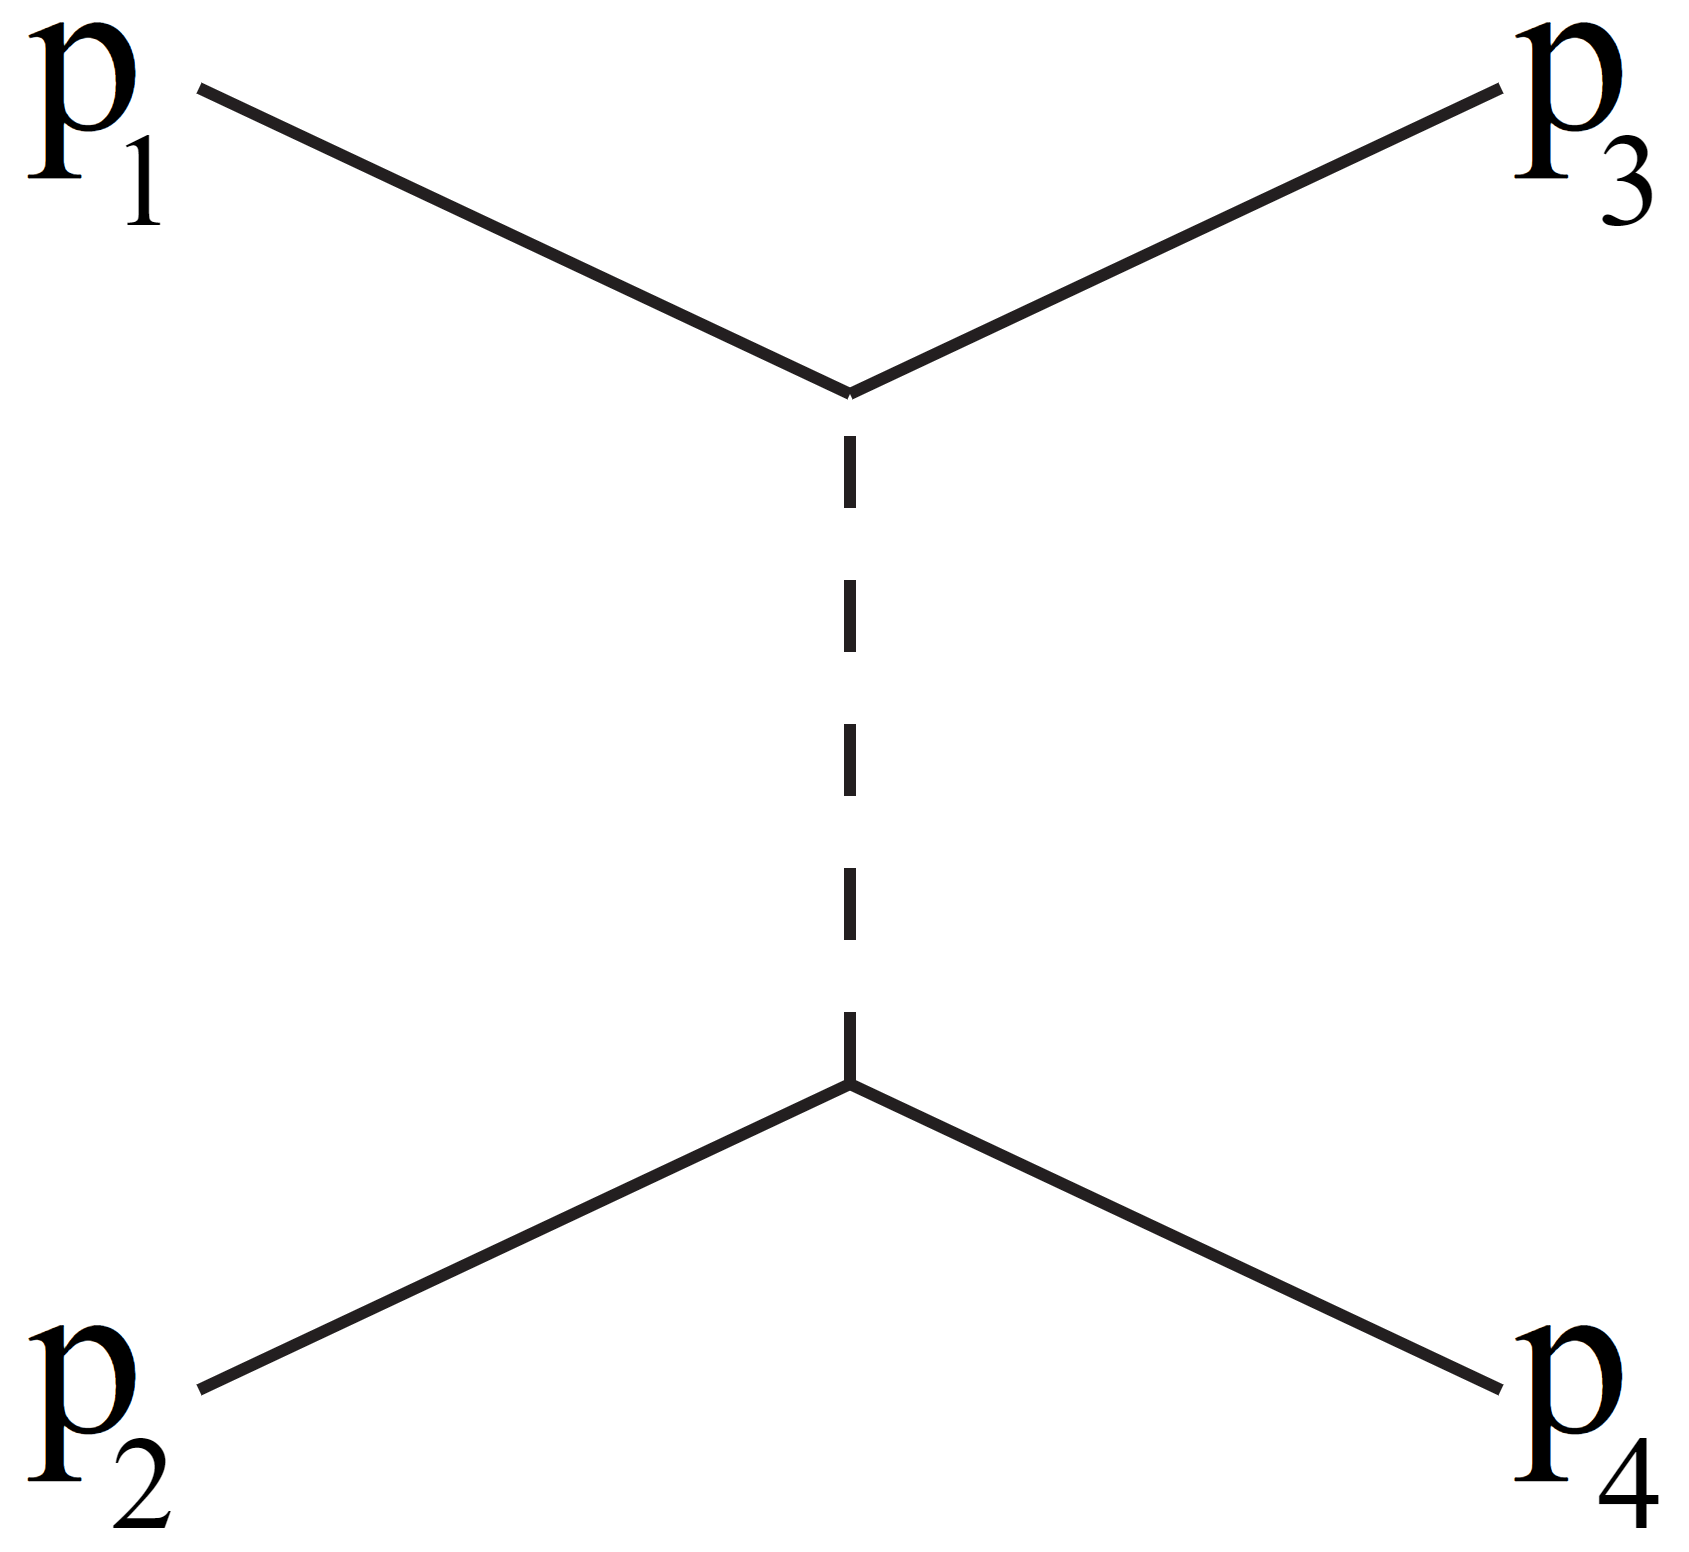
\includegraphics[width=0.35\columnwidth]{figures/Theory/TChannel.png}}
%	\caption{Feynman diagrams for (a) $s$-channel processes which could produce a new resonance and (b) $t$-channel background processes.
%	}
%	\label{fig:Feynman}
%\end{figure}

